\documentclass[12pt]{article}
\usepackage[utf8]{inputenc}
\usepackage[T1]{fontenc}
\usepackage{hyperref}
\usepackage[french]{babel}
\usepackage{graphicx}
\usepackage{wrapfig}
\usepackage[includeheadfoot, top=0.65in, bottom=0.65in, left=1in, right=1in, headheight=12pt, headsep=0.55in]{geometry}
\usepackage{titlesec}
\usepackage{float}


\setcounter{section}{-1}
\sloppy

\begin{document}

\begin{titlepage}
  \centering
  % Logos en haut de page
  \hfill
  \begin{minipage}{0.45\textwidth}
    \centering
    
\includegraphics[width=0.45\linewidth]{img/iia-logo.png}
  \end{minipage}
  \hfill
  \begin{minipage}{0.45\textwidth}
    \centering
    
\includegraphics[width=0.65\linewidth]{img/esiee-logo.png}
  \end{minipage}
  \vspace*{2cm}

  {\Huge Victor GIRAULT\par}
  \vspace*{2cm}
  {\Huge \textbf{Rapport d'activité}}\par
  \vspace{.5cm}
  {\LARGE 2ème année de Manager en ingénieurie informatique}\par
  \vspace{0.4cm}
  {\Large Option Lead Dev}\par
  \vfill
  % Bloc pour le tuteur
    
\includegraphics[width=0.2\textwidth]{img/logo-niji.png}\par
\vfill
  \begin{center}
    \textbf{Tuteur entreprise\\}
    Alban GRÉAU\\
    Architecte Solutions\\[2.5cm]
    \makebox[0pt][l]{\small Signature}\hspace{2cm}\rule{8cm}{0.5pt}\\
  \end{center}
  \vfill
  \begin{minipage}{0.55\textwidth}
    \raggedright
    {\large Institut Informatique Appliquée\par}
  \end{minipage}
  \hfill
  \begin{minipage}{0.4\textwidth}
    \raggedleft
    {\large Année scolaire 2024 - 2025\par}
  \end{minipage}
\end{titlepage}

\newpage
\tableofcontents
\thispagestyle{empty}
\newpage
\listoffigures
\thispagestyle{empty}
\newpage
\setcounter{page}{1}


\section{Introduction générale}
Ce mémoire a pour but de marquer l'aboutissement de mon parcours en master et représente une étape clé dans ma formation professionnelle. Il retrace le travail que j’ai effectué au sein de Niji, où j’ai eu l’opportunité de mettre en pratique les connaissances théoriques acquises au cours de mes études, tout en développant de nouvelles compétences dans un environnement professionnel exigeant. Cette année, j'ai évolué au sein du département DSF (Digital Software Factory) de l'antenne Rennaise de Niji, en tant qu'alternant "Ingénieur solutions".
\\\\
L’objectif de ce mémoire est de présenter de manière détaillée les missions qui m’ont été confiées, les méthodes et outils que j’ai utilisés, ainsi que les résultats obtenus. Il s’agit également de mettre en lumière les apprentissages tirés de cette expérience, tant sur le plan technique qu’humain, et de réfléchir à la manière dont cette immersion a enrichi ma compréhension des enjeux du secteur du développement informatique. Enfin, ce document vise à analyser les défis rencontrés et les solutions apportées, tout en proposant des pistes d’amélioration pour les projets futurs.
\\\\
À travers ce travail, je souhaite partager une vision à la fois critique et constructive de mon expérience en entreprise, en montrant comment elle a contribué à mon développement personnel et professionnel, et en soulignant son importance dans la construction de mon projet de carrière.
\\\\
J'ai intégré Niji en septembre 2024 en tant qu'alternant dans le cadre de ma deuxième année de formation de Manager en ingénieurie informatique (M2i) au sein de l'Institut Informatique Appliquée (IIA). À la suite de difficultés économiques et d'un manque de projets disponibles, j'ai été contraint de quitter l'entreprise d'alternance dans laquelle j'ai réalisé mes premières années en tant qu'alternant en développement informatique. Cette situation m'a poussé à rechercher une nouvelle entreprise pour poursuivre ma formation. Ayant réalisé mon année d'alternance de première année dans une petite entreprise de 4 employés, j'ai souhaité intégrer une entreprise de taille plus importante pour cette deuxième année afin de découvrir un environnement de travail différent et d'acquérir de nouvelles compétences. J'ai donc postulé chez Niji, une entreprise de services numériques (ESN) spécialisée dans le développement de solutions digitales. Après un entretien en présentiel avec Alban GRÉAU, et Kevin BELHADROUF, j'ai été retenu pour intégrer l'entreprise et travailler sur le projet "NijiSkills".
\newpage
\section{Présentation de l’entreprise}

\subsection{Présentation de Niji}

\begin{figure}[h!]
  \centering
  \begin{minipage}{0.4\textwidth}
    \centering
    
\includegraphics[width=0.7\textwidth]{img/logo-niji.png} 
    \caption{Logo de l'entreprise Niji}
  \end{minipage}
  \hspace{0.05\textwidth}
  \begin{minipage}{0.4\textwidth}
    \centering
    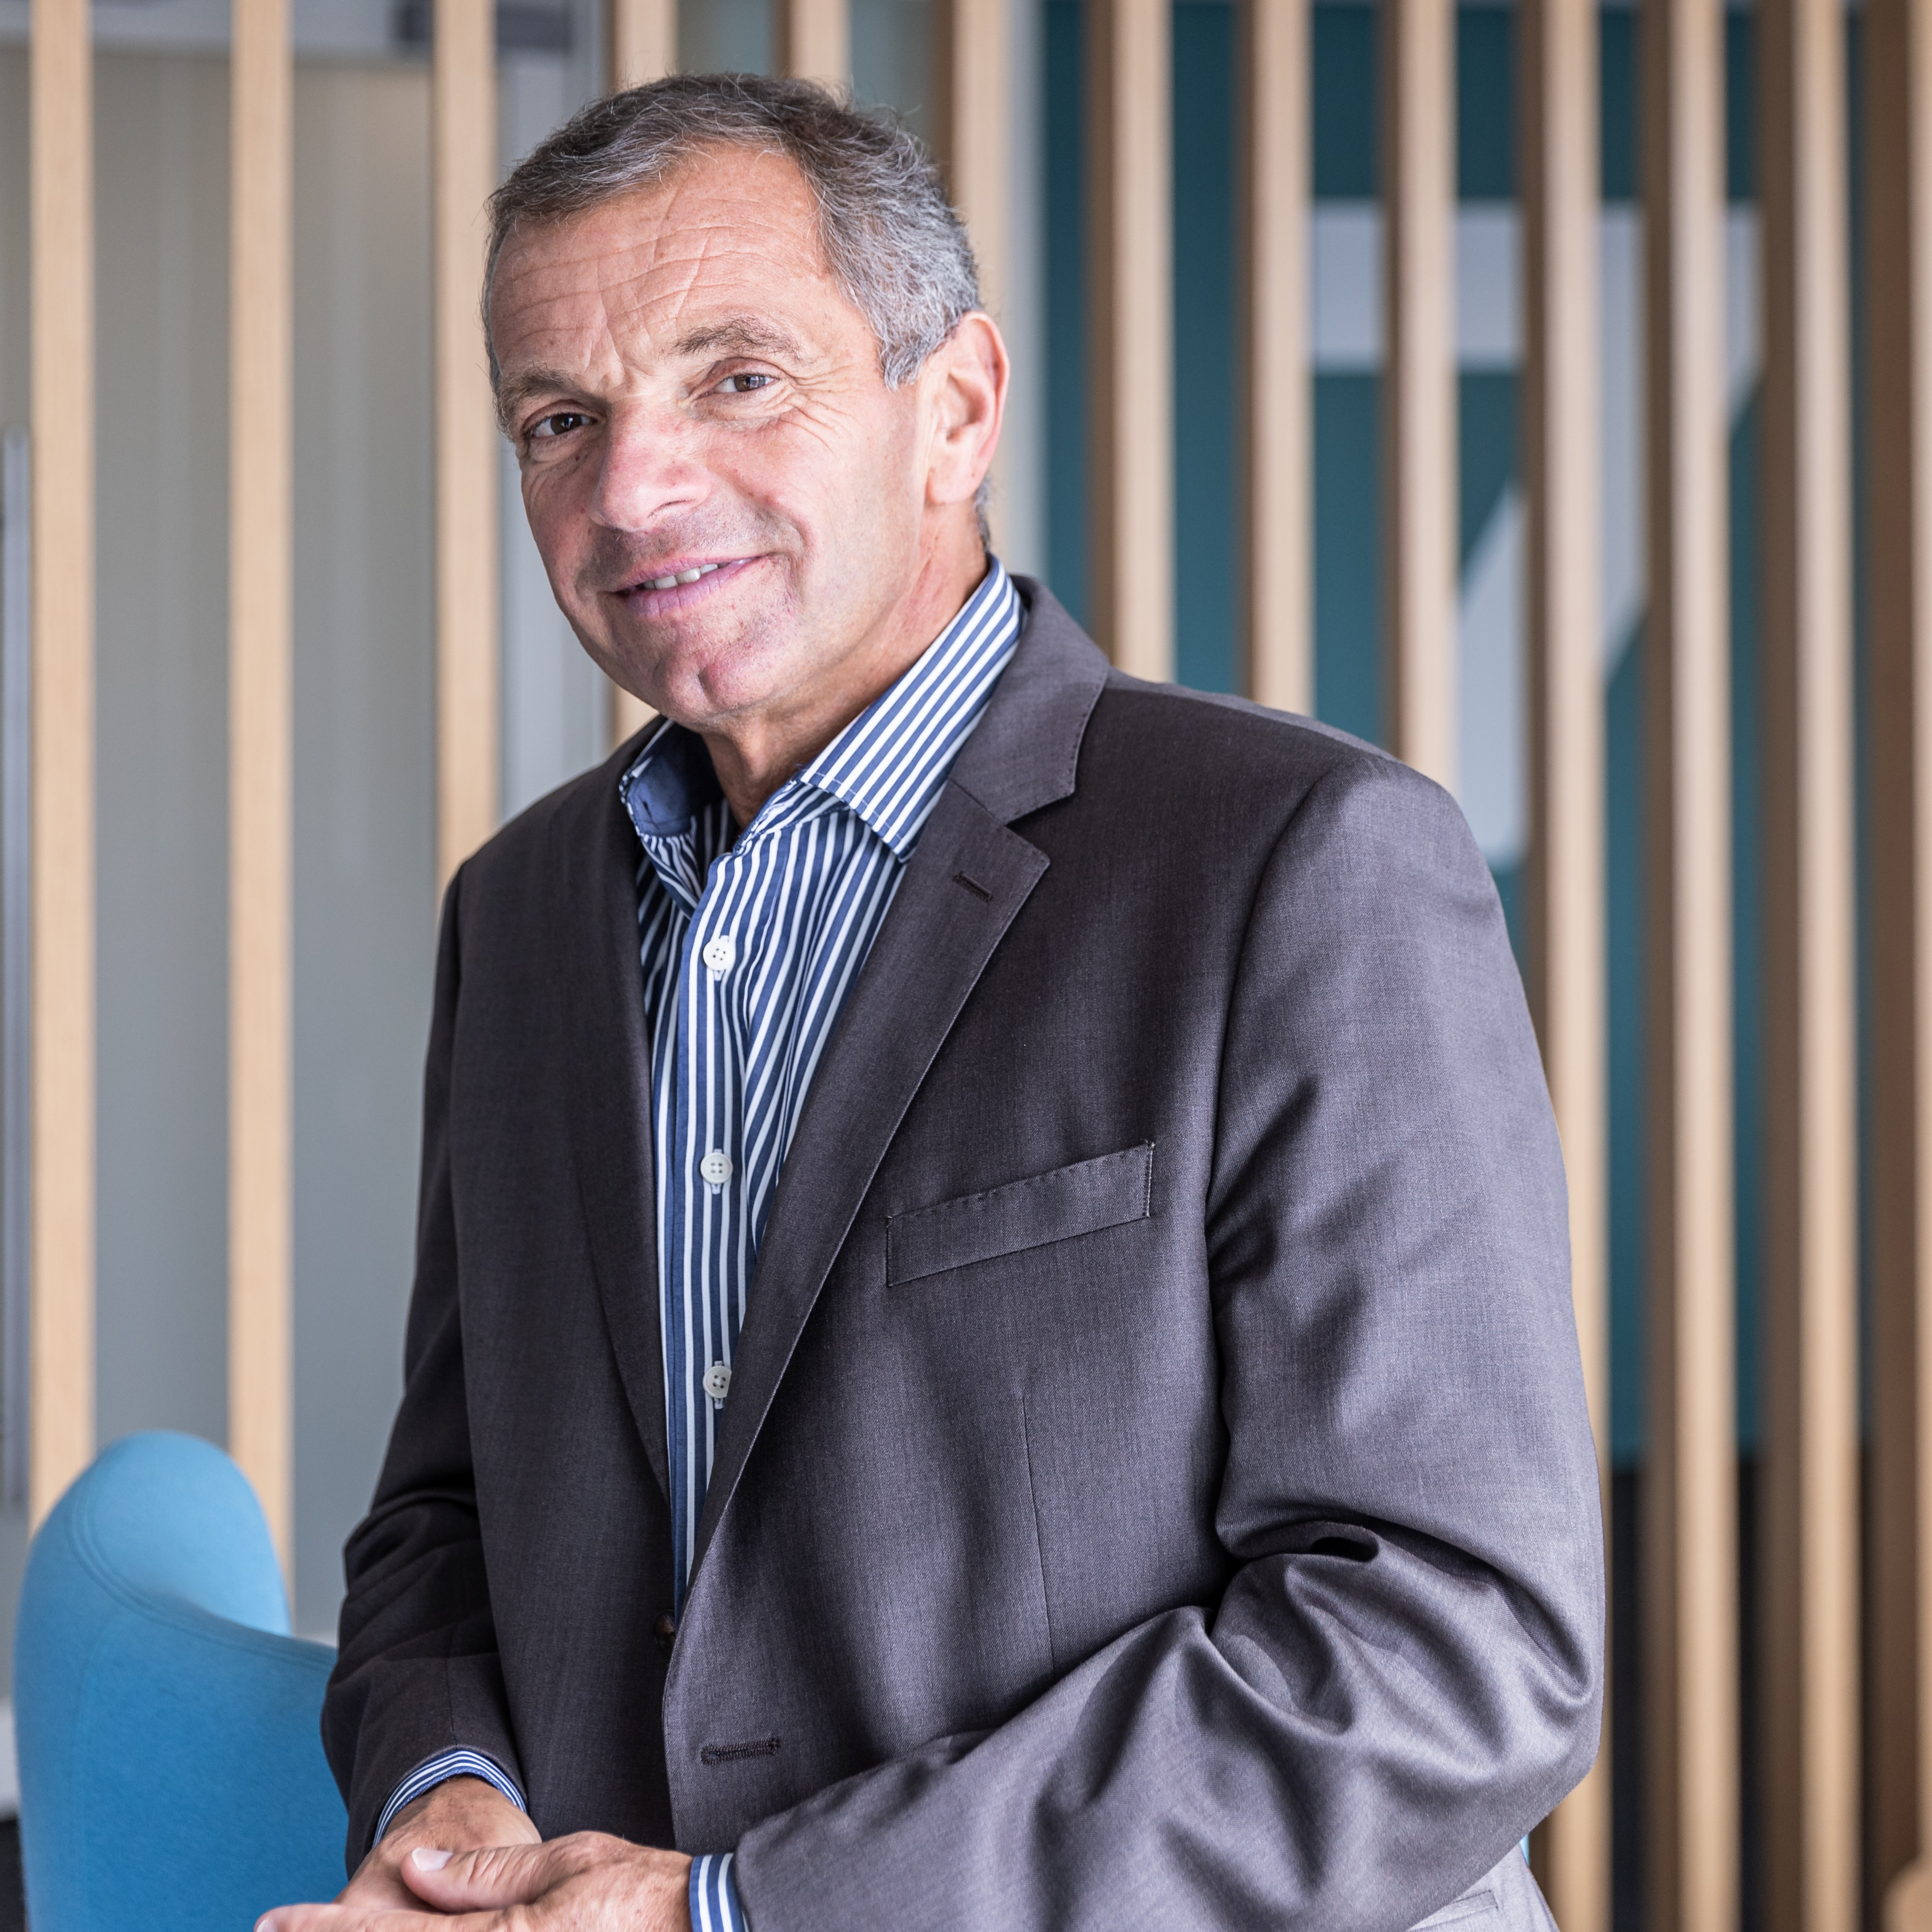
\includegraphics[width=0.7\textwidth]{img/hugues-meili.jpg}
    \caption{Hugues Meili}
  \end{minipage}
\end{figure}

\subsubsection{Création de l'entreprise}
Niji, qui signifie "arc-en-ciel" en japonais, est une entreprise co-fondée en septembre 2001 par Hugues Meili à Rennes. Niji est une ESN (Entreprise de service numérique) spécialisée dans le conseil, le design et le développement de solutions digitales pour des entreprises de toutes tailles. Depuis sa création, l'entreprise s'est imposée comme un acteur clé de la transformation numérique en France et à l'international.
\subsubsection{Positionnement et activités}
Niji se distingue par sa capacité à intervenir sur l'ensemble de la chaîne de valeur digitale. L'entreprise propose une large gamme de services adaptés aux besoins variés de ses clients. 
Tout d'abord, elle accompagne les entreprises dans la définition et la mise en œuvre de leur stratégie numérique. Cela inclut l'analyse des besoins métiers, l'identification des opportunités technologiques, et la conception de feuilles de route stratégiques alignées sur les objectifs de l'entreprise. Ce travail stratégique permet aux clients de mieux anticiper les évolutions du marché et de rester compétitifs.
\\\\
Ensuite, Niji excelle dans la conception de parcours utilisateurs innovants et intuitifs. Grâce à son expertise en design et en expérience utilisateur (UX/UI), l'entreprise crée des interfaces qui maximisent l'engagement des utilisateurs finaux. Cela inclut la réalisation de prototypes interactifs, des tests utilisateurs, et l'optimisation continue des interfaces pour garantir une expérience fluide et agréable.
\newpage
\noindent
Enfin, Niji développe et déploie des solutions technologiques sur mesure, intégrant les dernières innovations du marché. Cela comprend le développement d'applications web et mobiles, la mise en place de plateformes cloud, l'intégration de systèmes complexes, et l'automatisation des processus métiers. L'entreprise s'appuie sur des méthodologies agiles pour garantir une livraison rapide et de haute qualité, tout en s'adaptant aux besoins évolutifs des clients.
\\\\
En complément, Niji propose également des services de maintenance et de support technique pour assurer la pérennité des solutions déployées. Cela inclut la gestion des incidents, les mises à jour régulières, et l'accompagnement des équipes internes des clients pour une prise en main optimale des outils développés.
\\\\
Parmi les concurrents de Niji, on trouve de grands groupes comme Capgemini, Atos ou Sopra Steria, ainsi que des entreprises de taille moyenne comme Smile ou Devoteam à Rennes. Niji se distingue par sa capacité à combiner expertise technique et attention portée à l'utilisateur, ce qui lui permet de proposer des solutions innovantes et adaptées à chaque client. L'entreprise a aujourd'hui une bonne réputation dans le secteur du numérique, grâce à la qualité de ses projets et à sa capacité à innover. Niji est aussi reconnue pour son esprit collaboratif et sa faculté à s'adapter aux évolutions du marché technologique.
\subsubsection{Fonctionnement d'une ESN}
Une ESN (Entreprise de Services Numériques) est une entreprise spécialisée dans la fourniture de services informatiques et numériques. Elle intervient auprès de ses clients pour les accompagner dans leur transformation digitale, en proposant des solutions sur mesure adaptées à leurs besoins spécifiques. Le fonctionnement d'une ESN repose sur plusieurs éléments clés.
Tout d'abord, l'ESN recrute des experts dans divers domaines, tels que le développement logiciel, le design, la cybersécurité et le conseil. Ces experts sont ensuite affectés à des projets chez les clients, en fonction de leurs compétences et de leurs expériences. L'ESN agit en tant qu'intermédiaire entre ses collaborateurs et ses clients, en gérant les aspects administratifs, juridiques et financiers des missions.
\newpage
\subsubsection{Organisation interne}
Niji est structurée autour de plusieurs directions opérationnelles, chacune spécialisée dans un domaine particulier du numérique. Cette organisation permet de répondre efficacement aux besoins variés des clients et de favoriser la collaboration entre les équipes. Les principales directions sont :
\\
\begin{itemize}
    \item \textbf{DAF-SI} : Direction Administrative, Financière et Systèmes d'information
    \item \textbf{DRH} : Direction des Ressources Humaines
    \item \textbf{DCO} : Direction Commerciale
    \item \textbf{DCF} : Digital Consulting Firm (conseil stratégique et accompagnement à la transformation digitale)
    \item \textbf{DDA} : Digital Design Agency (design et expérience utilisateur)
    \item \textbf{DSF} : Digital Software Factory (développement logiciel, pôle Build et Run)
    \item \textbf{DST} : Digital Smart Technologies
    \item \textbf{DBS} : Digital Business Solutions
    \item \textbf{DCS} : Digital Cyber Security (Imineti by Niji, cybersécurité)
    \item \textbf{DDS} : Digital Data Solutions\\
\end{itemize}
\noindent
Chaque direction regroupe des experts dans son domaine et travaille en coopération avec les autres pour offrir des solutions complètes.
Par exemple, la DSF (Digital Software Factory) est responsable du développement des systèmes informatiques, tandis que la DDA se concentre sur le design et l’UX/UI.
La collaboration entre ces directions est facilitée par une culture d’entreprise basée sur la proximité, la transparence et l’innovation.
\\\\
L’entreprise valorise également la mobilité interne et la formation continue (ex : plateforme "Niji University"), permettant aux collaborateurs d’évoluer et de monter en compétences tout au long de leur parcours.
\subsubsection{Chiffres clés}
En 2025, Niji compte plus de 1400 collaborateurs répartis sur plusieurs sites en France et à l'international. L'entreprise, créée en 2001, réalise un chiffre d'affaires de 142 millions d'euros sur l'année 2024, avec une croissance de 20\% de son CA sur 5 ans, témoignant de sa solidité financière et de sa capacité à répondre aux attentes du marché.
\\\\
Niji accompagne plus de 300 clients, parmi lesquels figurent de grands groupes internationaux et nationaux, ainsi que des ETI et PME implantées sur l'ensemble des territoires. Cette diversité de clientèle illustre la capacité de l'entreprise à s'adapter à des besoins variés et à intervenir sur des projets d'envergure comme sur des missions plus ciblées.
\\\\
L'entreprise adresse plus de 25 secteurs d’activité, ce qui en fait un acteur multi-sectoriel reconnu. Niji intervient notamment dans les domaines de la banque, de l’assurance, des télécommunications, de l’énergie, du transport, de la distribution, de la santé, ou encore du secteur public, renforçant ainsi son expertise et sa polyvalence.
\\\\
Niji est présente dans dix sites en France, notamment à Rennes (siège social), Paris, Lyon, Lille, Nantes, Angers, Bordeaux et Nice. À l’international, l’entreprise dispose de bureaux à Singapour et Casablanca, renforçant ainsi sa dimension globale et sa capacité à accompagner des clients de toutes tailles, y compris des grands groupes internationaux. Récemment, Niji a également ouvert un nouveau site à Madrid, en Espagne, suite au rachat de l'entreprise Neo9, marquant une étape importante dans sa stratégie d’expansion européenne.
\subsubsection{La démarche RSE de Niji}
Niji s'engage activement dans une démarche de responsabilité sociétale des entreprises (RSE). Cela se traduit par des actions concrètes en faveur du développement durable, de la diversité et de l'inclusion. L'entreprise soutient également des initiatives locales et encourage ses collaborateurs à s'impliquer dans des projets solidaires.
\\\\
Dans une démarche de développement durable, Niji s'efforce chaque année de réduire son empreinte carbone. L'entreprise met en place des actions concrètes pour limiter la production de CO2 liée à ses activités, que ce soit par l'optimisation des déplacements professionnels, la mise en place du télétravail, la sensibilisation des collaborateurs aux éco-gestes ou encore l'amélioration de l'efficacité énergétique de ses infrastructures. Cette volonté de diminuer progressivement la fabrication de CO2 s'inscrit dans la politique RSE de Niji et témoigne de son engagement en faveur de la transition écologique.

\subsubsection{Perspectives d'avenir}

Niji ambitionne de poursuivre sa croissance en renforçant sa présence sur les marchés existants et en explorant de nouvelles opportunités.
Niji est en constante recherche de nouveaux talents pour accompagner sa croissance et répondre aux besoins variés de ses clients. L'entreprise recrute régulièrement des experts dans des domaines diversifiés, tels que le développement logiciel, la cybersécurité, le design UX/UI, ou encore l'intelligence artificielle. Cette stratégie de recrutement permet à Niji de rester à la pointe des innovations technologiques et d'offrir des solutions adaptées aux enjeux actuels.
\subsection{Le site de Rennes}
\subsubsection{Spécificités du site}
C'est en Bretagne, à Rennes, que Niji a ouvert sa première antenne en 2001. L'antenne Rennaise de Niji est aujourd'hui l'une des plus importantes de l'entreprise, avec plus de 300 collaborateurs. L'antenne Rennaise est un pôle d'excellence pour Niji, qui y développe des projets innovants et accompagne des clients de renom dans leur transformation digitale. Avec l'évolution de l'entreprise et les nouveaux bureaux ouverts dans les différentes villes de France, notamment à Paris, les bureaux bretons sont restés le siège social de l'entreprise notamment pour des raisons historiques mais surtout pour l'amour de la Bretagne du fondateur.
\\\\
Les bureaux de Niji à Rennes sont situés à EuroRennes, une nouvelle zone d'activité dynamique, à proximité de la gare et du centre-ville. S'étalant sur 3 étages, les locaux sont modernes et spacieux, offrant un cadre de travail agréable et stimulant pour les collaborateurs. Les bureaux Rennais sont équipés de salle de réunions, de cabines insonorisées, d'un espace de restauration avec une terrasse extérieure. Les espaces de travail sont modulables et permettent aux équipes de s'organiser selon leur besoins. 
\subsubsection{Imineti by Niji}
\begin{wrapfigure}{l}{0.32\textwidth}
    \centering
    
\includegraphics[width=0.85\linewidth]{img/imineti.jpg} 
    \caption{Logo de Imineti by Niji}
    \label{fig:wrapfig}
\end{wrapfigure}
Imineti by Niji est une branche de l'entreprise Niji spécialisée dans la gestion des risques numériques et la cybersécurité. Elle combine conseil en cybersécurité et expertise technique pour aider les entreprises à définir et mettre en œuvre des stratégies de sécurité efficaces. Imineti by Niji accompagne ses clients tout au long du processus, de l'analyse des risques et des tests d'intrusion jusqu'à la présentation des recommandations devant les comités de direction. L'objectif est de fournir une vision cohérente et à long terme de la sécurité, en aidant les entreprises à formaliser et à appliquer des règles de sécurité adaptées à leurs besoins.
\\
Imineti by Niji est localisé à Rennes, au sein de l'antenne Rennaise de Niji. Pour des raisons de sécurité et de confidentialité, l'accès aux bureaux d'Imineti est restreint. Si une personne non autorisée souhaite entrer dans les locaux d'Imineti, elle doit remplir une feuille en spécifiant son identité, son heure d'arrivée et de départ. Ainsi, les équipes d'Imineti peuvent savoir qui est présent dans les locaux à tout moment. De plus, l'accès aux bureaux d'Imineti est sécurisé par des badges magnétiques, ce qui permet de contrôler les entrées et sorties des personnes autorisées.
\newpage
\subsection{Le département DSF (Digital Software Factory)}
Durant mon contrat d'apprentissage avec Niji, j'ai intégré la direction opérationnelle DSF (Digital Software Factory). Ce département est en charge du développement des systèmes informatiques des clients de Niji.
\\\\
Le département est constitué de deux pôles principaux : le pôle "Build" et le pôle "Run". Le pôle "Build" est en charge de la conception et du développement de solutions digitales pour les clients de Niji, tandis que le pôle "Run" assure la maintenance et l'exploitation de projets déjà déployés et en production. Le pôle "Run" est également en charge de la gestion des incidents et des demandes de support technique.
\\\\
Les clients du département DSF sont variés, allant des grandes entreprises aux PME, et couvrent de nombreux secteurs d'activité. 
Alban GRÉAU, mon tuteur, est notamment architecte solution pour les projets de développement d'une application mobile de e-commerce pour Lacoste ainsi que pour un projet de la banque BNP.
\subsection{Mon rôle en tant qu’alternant}
\subsubsection{Poste et missions}
Durant mon contrat d'apprentissage avec Niji, j'ai intégré la direction opérationnelle DSF (Digital Software Factory) et ai été affecté au poste de "Ingénieur solutions".
Je n'ai pas intégré d'équipe existante en particulier. En effet, j'ai été affecté à un projet interne de l'entreprise dont le développement n'avait pas encore débuté. Aucune équipe n'a donc été formée pour ce projet. Cependant, j'ai eu l'occasion de travailler avec plusieurs collaborateurs de Niji pour la mise en place de ce projet et son développement :
\paragraph{Alban GRÉAU} est le responsable du projet NijiSkills. Il a été mon tuteur durant mon année d'alternance et m'a accompagné tout au long de mon parcours chez Niji. Alban est architecte solution à Niji Rennes, et possède une solide expérience dans la gestion de projets digitaux. Il a su me guider et me conseiller dans mes missions, tout en me laissant une certaine autonomie pour développer mes compétences et donner mon avis sur certaines solutions.
\paragraph{Olivier DELALANDE} est un développeur React au sein de l'équipe DSF à Niji Paris. Il m'a rejoint sur le projet NijiSkills en tant que développeur en Avril 2025 afin d'apporter son expertise technique et de m'aider à développer le projet. Olivier a une forte expérience dans le développement d'application web avec React et a su me guider quant aux bonnes pratiques de développement. Il est intervenu notamment sur la partie de synchronisation des compétences entre l'application Nijskills et DoYouBuzz, une plateforme de création de CV en ligne.
\\\\
Ma mission principale au sein de Niji, pour ma période d'alternance, à été le développement de l'application interne NijiSkills. Cette application a pour but de centraliser les compétences des collaborateurs de Niji, de les aider à se former en leur proposant des parcours de compétences à acquérir pour évoluer dans leur carrière, et de les accompagner dans leur montée en compétences. NijiSkills est un projet ambitieux qui vise à améliorer la gestion des compétences au sein de l'entreprise et à favoriser le développement professionnel des collaborateurs.
\subsubsection{Objectifs professionnels de l’alternance}
Au début de mon alternance chez Niji, je voulais découvrir le fonctionnement d’une grande entreprise. Après une expérience dans une petite structure, il était important pour moi de comprendre comment s’organisent les équipes, comment se passe la communication entre les différents services et comment sont gérés les projets à grande échelle. Cette immersion m’a permis d’avoir une vision plus large du secteur du numérique et de découvrir les enjeux et les défis auxquels sont confrontées les grandes entreprises.
\\\\
Un autre objectif était de renforcer mes compétences techniques en travaillant sur de nouvelles technologies. Le développement de l’application NijiSkills m’a permis d’apprendre de nouveaux outils et frameworks, tout en les utilisant directement dans un contexte professionnel. Cette expérience m’a poussé à sortir de ma zone de confort, à chercher des solutions par moi-même et à demander de l’aide à mes collègues si besoin.
J'ai donc dû apprendre ces technologies directement en développant l'application NijiSkills, sans passer par la réalisation de projets d'entraînement ou de tests préalables, ce qui m'a permis d'acquérir des compétences concrètes en situation réelle.
Mais aussi, j'ai pu approfondir mes connaissances en React, TypeScript et Node.js, des technologies que je n'avais pas eu l'occasion d'utiliser en profondeur auparavant.
\\\\
Enfin, l’un des objectifs majeurs de mon alternance était de pouvoir poursuivre ma carrière chez Niji à l’issue de cette expérience, en obtenant une proposition de contrat. J’ai donc mis un point d’honneur à démontrer mon sérieux, mon implication et ma capacité à mener à bien un projet complet, afin de convaincre l’entreprise de m’accorder sa confiance pour la suite de mon parcours professionnel.
\newpage
\section{Présentation de la mission : développement de NijiSkills}
\subsection{Contexte du projet}
Dans cette section, je vais présenter le contexte dans lequel s’inscrit ma mission au sein de Niji, ainsi que les objectifs qui ont guidé le développement de l’application NijiSkills. Comprendre l’environnement, les enjeux et les attentes liés à ce projet est essentiel pour appréhender les choix techniques et organisationnels qui ont été faits tout au long de la mission. Cette présentation permettra de mettre en lumière les besoins auxquels l’application devait répondre, les contraintes rencontrées, ainsi que la démarche adoptée pour concevoir une solution adaptée aux spécificités de l’entreprise et de ses collaborateurs.
\subsubsection{Origine du besoin}
L'origine du besoin pour le projet NijiSkills provient d'abord du constat d'Alban GRÉAU, architecte solution et responsable du projet, qu'il devenait compliqué d'évaluer un candidat lors d'un entretien avec une simple grille de questions et une note pour chaque question. Cette méthode, bien que répandue, montrait rapidement ses limites : elle ne permettait pas de refléter fidèlement la diversité et la profondeur des compétences d'un candidat, ni de prendre en compte les parcours d'apprentissage ou les évolutions de carrière possible. Face à cette difficulté, Alban a exprimé le besoin de disposer d'un outil plus structurant et plus précis pour cartographier les compétences, suivre leur évolution et faciliter l'évaluation lors des entretiens. Ce constat a servi de point de départ à la réflexion autour de la création d'une application dédiée, capable de centraliser et de valoriser les compétences des collaborateurs tout en offrant une meilleure visibilité sur les axes de progression possibles.
\\\\
Dans ce contexte, la mise en place d’un outil interne permettant de cartographier les
compétences, de faciliter la montée en compétences des équipes et d’optimiser l’affectation
des collaborateurs sur les projets. L’objectif était également de proposer un accompagnement
personnalisé aux collaborateurs dans leur évolution professionnelle, en leur offrant une
meilleure visibilité sur les compétences à acquérir pour atteindre leurs objectifs de carrière.
\\\\
Le projet s’inscrit donc dans une démarche d’amélioration continue des processus RH
et de développement des talents, tout en répondant à des enjeux opérationnels concrets :
mieux connaître les expertises internes, anticiper les besoins en formation, et renforcer
l’attractivité de Niji en tant qu’employeur. Le développement de NijiSkills s’est appuyé
sur une collaboration étroite entre les équipes techniques, les ressources humaines et les
managers, afin de concevoir une solution adaptée aux attentes de l’ensemble des parties
prenantes.
\subsubsection{Objectifs de l’application}
L’application NijiSkills vise avant tout à centraliser l’ensemble des compétences des collaborateurs de Niji dans un outil unique. Cette centralisation permet de disposer d’une cartographie précise et à jour des expertises présentes au sein de l’entreprise. Grâce à cette visibilité, il devient plus simple pour les managers et les équipes RH d’identifier les forces internes, de repérer les besoins en formation, et d’optimiser l’affectation des collaborateurs sur les projets en fonction de leurs compétences réelles.
\\\\
Un autre objectif majeur du projet est d’explorer et d’expérimenter de nouvelles technologies qui n’étaient pas encore utilisées chez Niji. Le choix de Next.js pour le développement du front-end et de l’API, associé à TailwindCSS pour le design et à Prisma comme ORM pour la gestion de la base de données PostgreSQL, s’inscrit dans une démarche d’innovation technique. Cette volonté d’adopter des outils modernes permet non seulement d’enrichir la culture technologique de l’entreprise, mais aussi de préparer l’équipe à de futurs projets nécessitant ces compétences.
\\\\
Enfin, NijiSkills ambitionne de proposer un accompagnement personnalisé aux collaborateurs dans leur évolution professionnelle. En offrant une vision claire des compétences à acquérir et des parcours de progression possibles, l’application facilite la montée en compétences et encourage le développement continu. Elle contribue ainsi à renforcer l’attractivité de Niji en tant qu’employeur et à fidéliser les talents en leur offrant des perspectives d’évolution concrètes et adaptées à leurs aspirations.
\subsubsection{Contraintes techniques et fonctionnelles}
Il n’existe pas de contrainte technique majeure imposée par l’environnement ou le contexte du projet NijiSkills. Les contraintes rencontrées sont principalement issues de choix délibérés réalisés par Alban GRÉAU, responsable du projet, dans une démarche d’exploration de nouvelles technologies et de méthodes de développement. L’objectif était de sortir des sentiers battus et d’expérimenter des outils et frameworks encore peu utilisés chez Niji, afin d’enrichir la culture technique de l’équipe et d’ouvrir de nouvelles perspectives pour les futurs projets.
\\\\
Ainsi, le choix de la stack technique (Next.js, TailwindCSS, Prisma, PostgreSQL) n’a pas été dicté par des exigences externes ou des limitations techniques, mais bien par la volonté de tester des solutions innovantes et de se confronter à des problématiques inédites. Cette approche a permis de découvrir de nouvelles façons de concevoir et de développer une application complète, tout en favorisant l’apprentissage continu et l’adaptabilité.
\\\\
Il existait toutefois une contrainte technique importante : il fallait proposer une visualisation des compétences sous forme de "carte", à la manière de ce que propose le site roadmap.sh. Cela impliquait de mettre en place un "canvas" interactif permettant d’afficher, de relier et de manipuler graphiquement les différentes compétences, afin d’offrir une vue d’ensemble claire et intuitive. Ce besoin a fortement orienté les choix techniques et la conception de l’interface utilisateur.
\\\\
En conséquence, les contraintes du projet étaient davantage organisationnelles et pédagogiques que techniques. Il s’agissait de s’approprier rapidement des technologies inconnues, de mettre en place des bonnes pratiques de développement dans un contexte d’apprentissage, et de garantir la qualité du code tout en assurant l’avancement du projet. Ce cadre a offert une grande liberté dans la conception de l’application, tout en posant le défi de structurer le projet de manière efficace et pérenne.
\subsection{Cadrage du projet}
\subsubsection{Méthodologie utilisée}
Habituellement, Niji travaille en mode agile, en mettant en place des méthodologies telles que Scrum ou Kanban, avec des équipes projet complètes, des rituels réguliers (sprints, daily meetings, rétrospectives) et un suivi itératif de l'avancement. Cependant, dans le cadre du développement de NijiSkills, le contexte était particulier : n'étant pas intégré à une équipe projet complète et travaillant principalement en autonomie, il n'a pas été pertinent d'appliquer une méthodologie agile classique. Pour assurer un suivi rigoureux de l'avancement et de la priorisation des tâches, l'outil Jira a été utilisé tout au long du projet. Jira a permis de lister, organiser et suivre l'ensemble des tâches à réaliser. Cet usage a facilité la communication avec mon tuteur et les intervenants ponctuels, tout en offrant une visibilité claire sur la progression du développement de l'application.
\\
\begin{figure}[H]
  \centering
  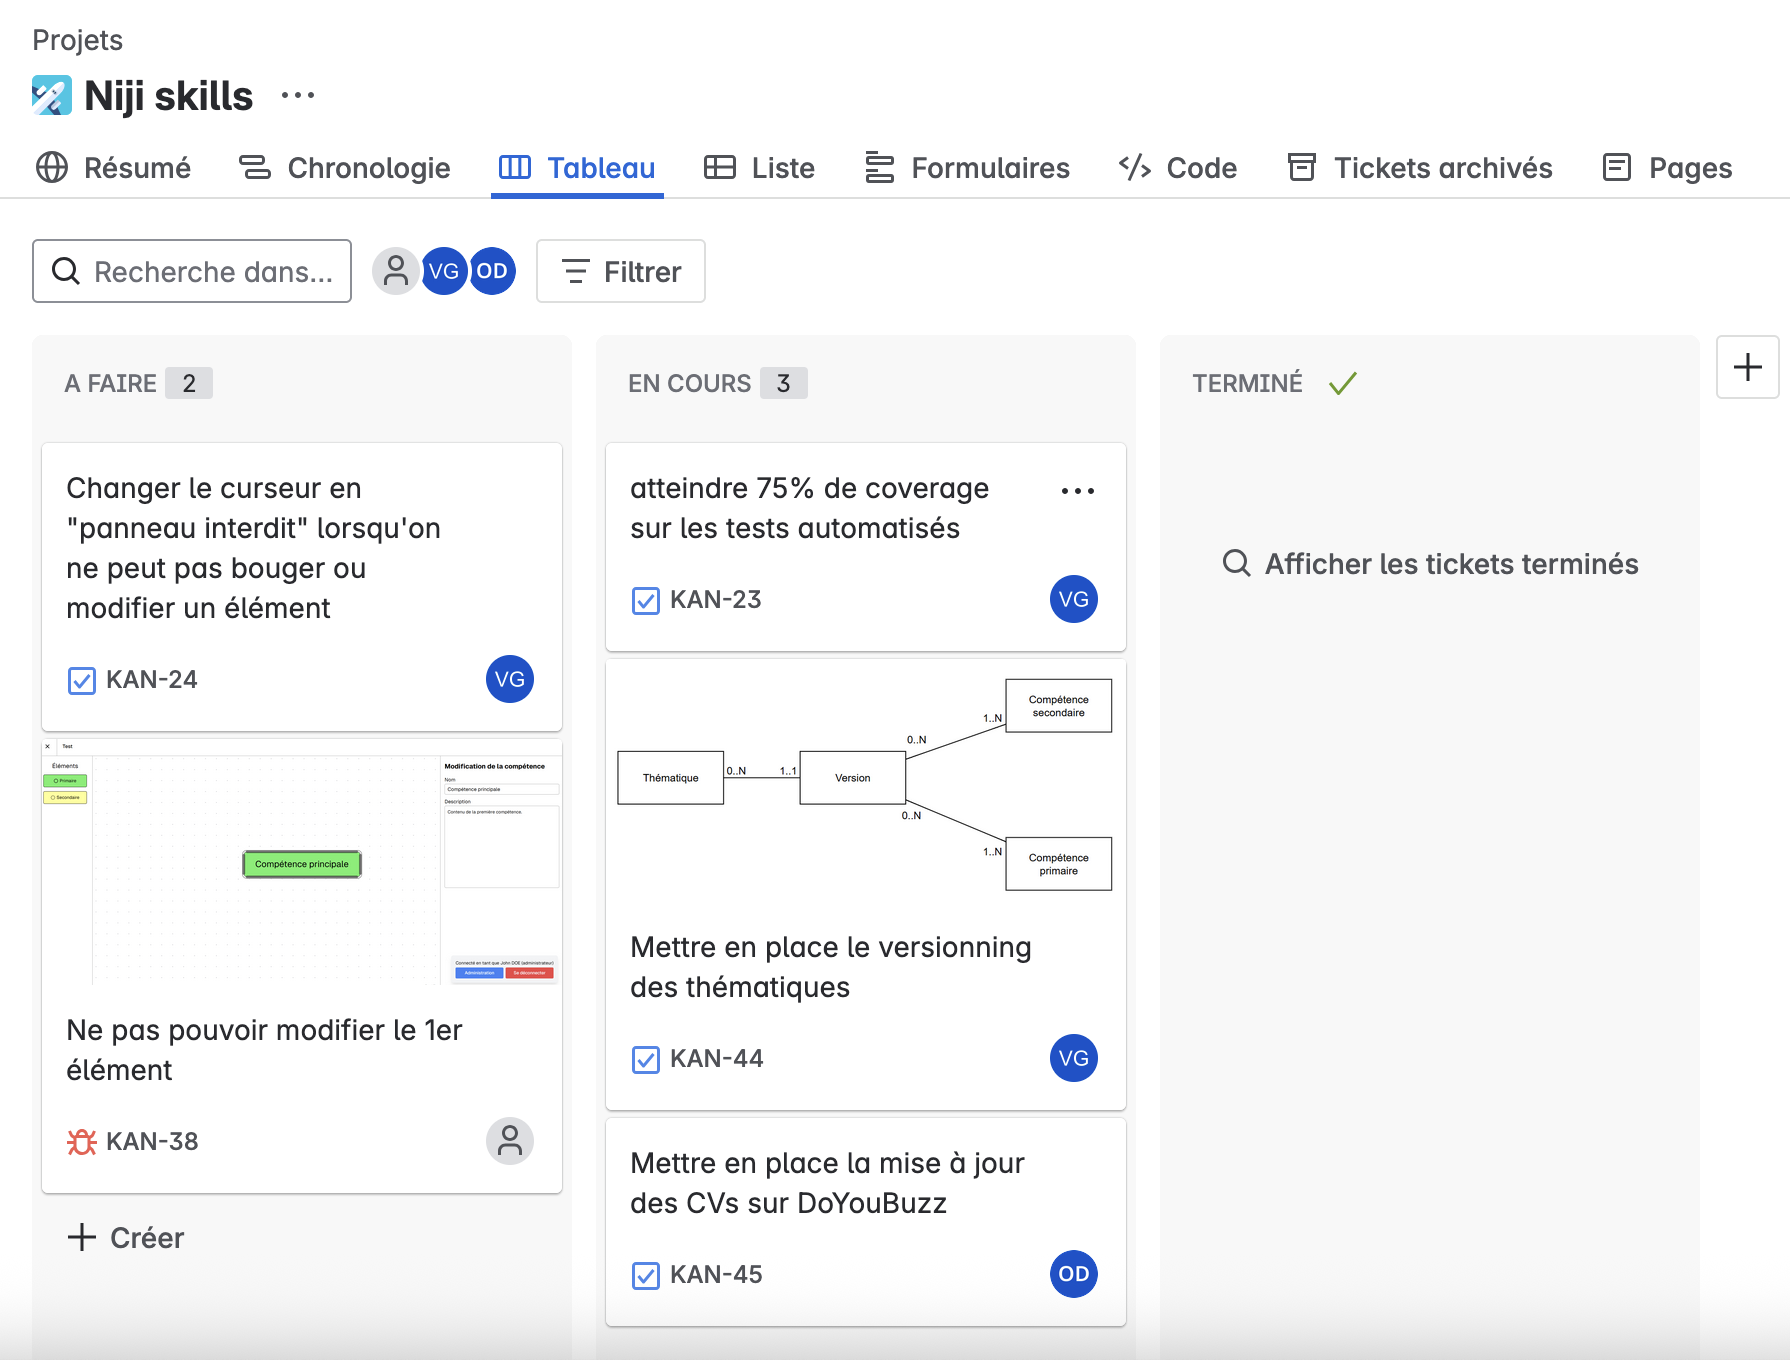
\includegraphics[width=0.8\textwidth]{img/jira.png}
  \caption{Exemple d'utilisation de Jira pour le suivi des tâches du projet NijiSkills}
\end{figure}

\subsubsection{Planification et priorisation des tâches}
Le découpage des tâches du projet NijiSkills s’est fait par paliers de réalisation, chaque tâche correspondant à une fonctionnalité majeure de l’application. Nous avons ainsi débuté par les fondations techniques indispensables, telles que la mise en place du SSO Microsoft, la connexion à la base de données, l’intégration de la CI (Continuous Integration) et l’ajout des premiers tests unitaires avec Jest. Ce premier palier a permis de garantir un socle technique robuste et sécurisé, sur lequel les développements ultérieurs ont pu s’appuyer.
\\\\
Une fois ces éléments essentiels en place, le découpage des tâches a évolué pour accompagner la montée en complexité de l’application. Chaque nouvelle tâche représentait alors soit l’ajout d’une nouvelle fonctionnalité (feature), soit une amélioration ou une correction du fonctionnement existant. Par exemple, la gestion du versionning des thématiques, l’ajout du rôle manager, ou encore la mise en place de la gestion des utilisateurs par les managers ont constitué des étapes importantes dans l’évolution du projet. Ce découpage progressif a permis d’avancer de manière structurée, en validant chaque étape avant de passer à la suivante.
Il est important de souligner que les tâches n’étaient pas associées à des dates limites strictes. Au lieu d’imposer des deadlines fixes, nous avons préféré organiser les tâches selon leur niveau d’urgence et leur impact sur l’avancement global du projet. Cette approche a permis de rester flexible et de s’adapter aux imprévus, tout en assurant que les priorités les plus critiques étaient traitées en premier. La classification par urgence a également facilité la communication avec les parties prenantes et permis de réagir rapidement en cas de besoin.
\\\\
En résumé, la planification du projet s’est appuyée sur un découpage par paliers fonctionnels, une priorisation par urgence plutôt que par échéance, et une adaptation continue aux besoins et aux retours des utilisateurs. Cette organisation a favorisé la progression régulière du développement tout en maintenant une grande réactivité face aux évolutions du projet.
\subsubsection{Collaboration inter-équipes}
La grande force de Niji est qu'elle possède de nombreux pôles d'expertise, ce qui permet de collaborer avec des experts dans différents domaines. Ainsi, pour le développement de l'application NijiSkills, j'ai pu bénéficier de l'expertise d'Alban GRÉAU, mon tuteur. Alban a su me guider dans la conception et le développement de l'application, en m'apportant son expérience et ses conseils sur les choix techniques à adopter. J'ai aussi pu travailler avec Olivier DELALANDE, un développeur React de l'équipe DSF à Niji Paris. Olivier a apporté son aide technique et m'a aidé à développer certaines fonctionnalités de l'application, notamment la synchronisation des compétences entre NijiSkills et DoYouBuzz.
\\\\
J'ai aussi pu travailler avec l'équipe chargée des tests à Niji. Premièrement, Antoine VALLERY, un testeur de l'équipe DSF à Rennes, a testé plusieurs aspects globaux de l'application Nijiskills grâce à une documentation utilisateur que j'ai rédigée. Il a pu ainsi vérifier que l'application répondait aux besoins fonctionnels et qu'elle était conforme aux attentes des utilisateurs. 
\\\\
J'ai aussi pu discuté avec Tanguy MICHEL pour la mise en place de tests E2E \footnote{End to end:  tests automatisés qui valident le bon fonctionnement d’une application dans son ensemble, en simulant le parcours complet d’un utilisateur final } avec Playwright. Tanguy est un développeur de l'équipe DSF à Rennes, et il m'a aidé à comprendre comment mettre en place des tests automatisés pour vérifier le bon fonctionnement de l'application dans son ensemble. Ces tests permettront de s'assurer que les différentes fonctionnalités de NijiSkills fonctionnent correctement et que l'application est stable. Il m'a aussi expliquer comment mettre en place Playwright dans le projet, et comment l'utiliser pour écrire des tests E2E.
\\\\
J'ai aussi eu à contacter Dimitri GOULIARMIS, un developpeur Flutter de l'équipe DSF à Rennes, pour qu'il puisse créer une première thématique "Flutter" de test pour pouvoir l'utiliser pendant un prochain entretien.

\subsection{Architecture technique}
\subsubsection{Choix de la stack}

L’architecture technique de l’application NijiSkills repose sur une stack moderne et performante. Le choix de Next.js avec TypeScript permet de bénéficier d’un framework robuste pour le développement à la fois du front-end et de l’API, offrant ainsi une cohérence et une maintenabilité accrues du code. L’utilisation de TailwindCSS facilite la création d’interfaces utilisateur réactives et personnalisées, tout en accélérant le processus de développement grâce à ses classes utilitaires. La base de données PostgreSQL, reconnue pour sa fiabilité et ses performances, est gérée via l’ORM Prisma, qui simplifie les interactions avec la base et améliore la productivité des développeurs. Enfin, l’ensemble de l’application est conteneurisé avec Docker, ce qui garantit la portabilité, la reproductibilité des environnements et facilite le déploiement sur différents serveurs ou plateformes cloud. Cette combinaison de technologies assure à la fois flexibilité, évolutivité et sécurité pour le projet.
\begin{figure}[H]
  \centering
  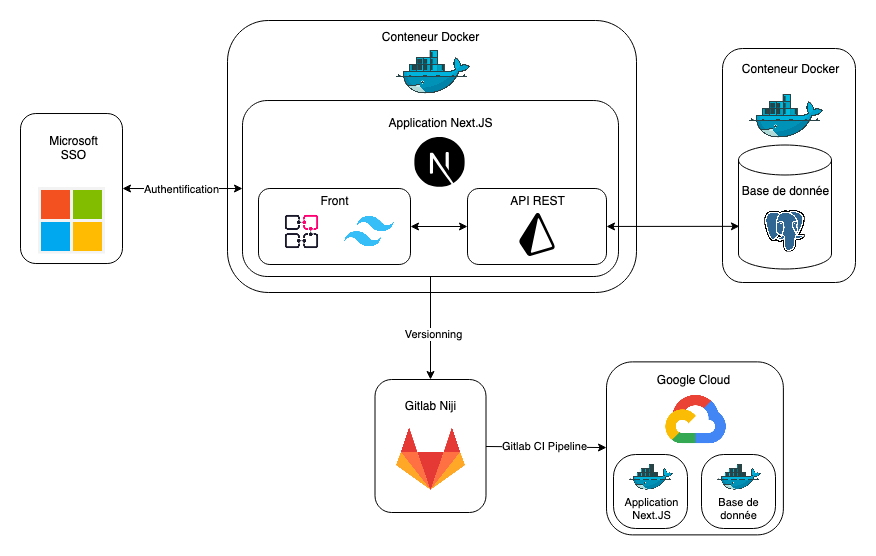
\includegraphics[width=0.85\textwidth]{img/archi.png}
  \caption{Architecture du projet}
\end{figure}
\noindent
Cette stack technique à aussi été choisie car ce sont des technologies que Niji n'utilisait pas encore, et qui sont donc nouvelles pour l'entreprise. L'objectif était de découvrir de nouvelles technologies et de les expérimenter dans un projet concret, afin de les maîtriser, de comptendre leurs avantages et inconvénients, et de potentiellement pouvoir les utiliser dans de futurs projets.
\newpage
\subsubsection{Authentification SSO Microsoft}
L’application NijiSkills étant destinée exclusivement aux collaborateurs de Niji, il était impératif de restreindre l’accès à la plateforme afin de garantir la confidentialité des données et d’éviter toute utilisation non autorisée. Pour répondre à cette exigence, la mise en place d’une authentification SSO (Single Sign-On) via Microsoft a été choisie. Cette solution permet de s’assurer que seuls les salariés disposant d’un compte Microsoft professionnel Niji peuvent se connecter à l’application, consulter ou compléter leurs compétences. L’authentification SSO offre également une expérience utilisateur fluide, en évitant la multiplication des identifiants et mots de passe, tout en renforçant la sécurité globale de l’accès à l’outil.
\\\\
La mise en place d’une connexion SSO avec Microsoft nécessite plusieurs étapes techniques. Tout d’abord, il faut enregistrer l’application NijiSkills auprès de l’Azure Active Directory (Azure AD) de Niji, en créant une nouvelle application dans le portail Azure. Cette opération permet d’obtenir un identifiant client (Client ID) et un secret d’application (Client Secret), qui serviront à authentifier l’application auprès des services Microsoft. Ensuite, il convient de configurer les redirections d’URL autorisées, afin que Microsoft puisse renvoyer l’utilisateur vers l’application après authentification.
\begin{figure}[H]
  \centering
  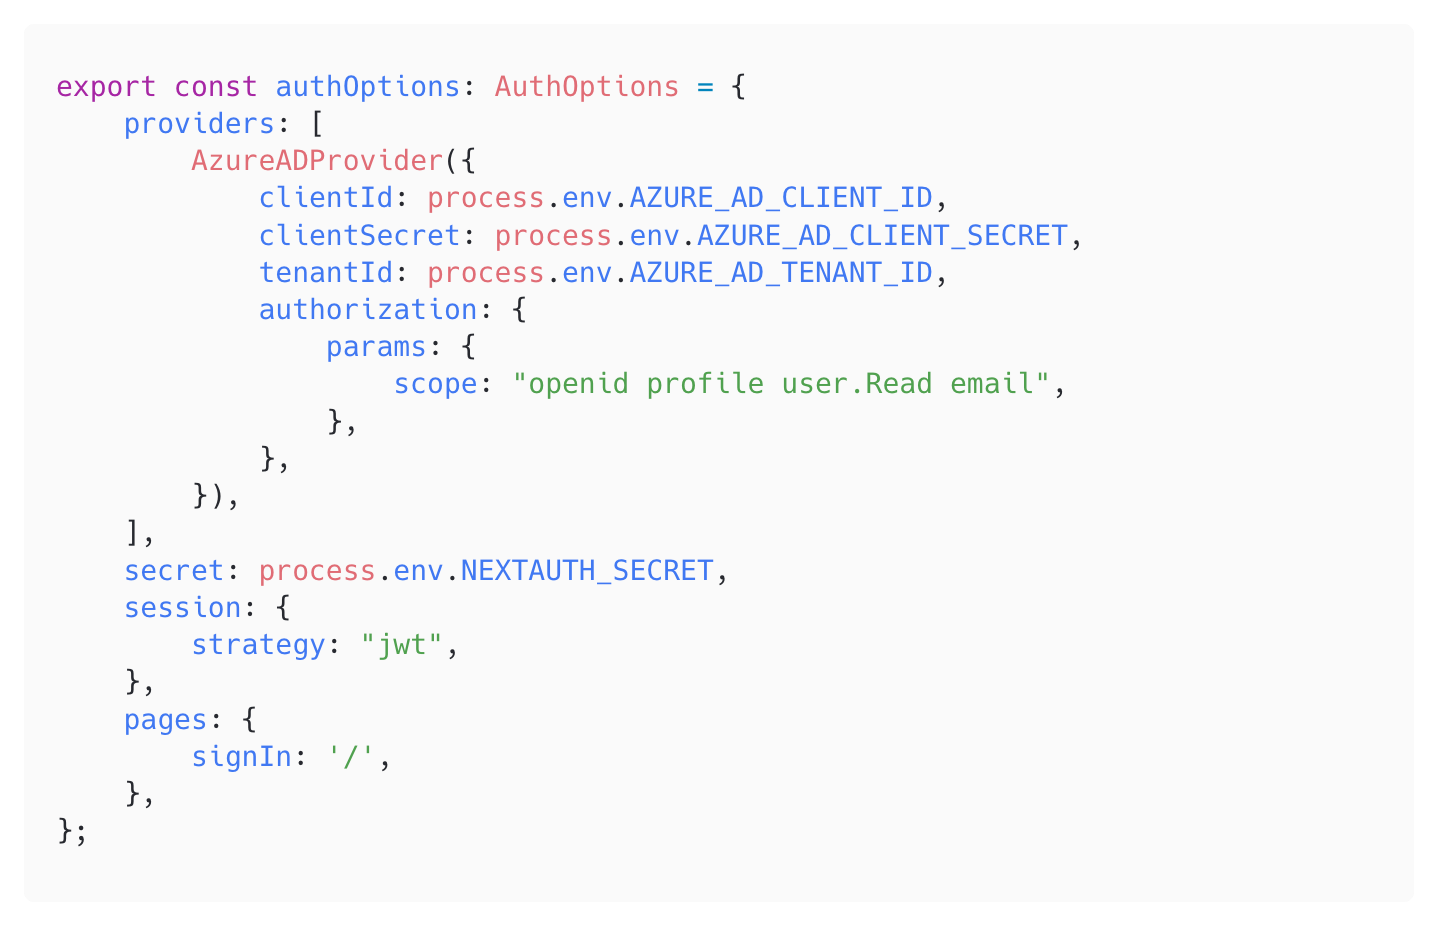
\includegraphics[width=0.85\textwidth]{img/code-auth.png}
  \caption{Exemple de code pour l'intégration de l'authentification SSO Microsoft avec NextAuth.js}
\end{figure}
\noindent
Côté application, il est nécessaire d’intégrer une bibliothèque compatible avec le protocole OAuth 2.0 et OpenID Connect, comme \texttt{next-auth} pour Next.js et de configurer les options avec les identifiants récupérer précedemment. Cette bibliothèque facilite la gestion du flux d’authentification, la récupération des informations de l’utilisateur (nom, email, etc.) et la gestion des sessions. Lorsqu’un utilisateur tente de se connecter, il est redirigé vers la page de connexion Microsoft, où il doit s’authentifier avec ses identifiants professionnels. Une fois l’authentification validée, Microsoft renvoie un jeton d’accès (access token) à l’application, qui peut alors vérifier l’identité de l’utilisateur et lui accorder l’accès à la plateforme.
\\\\
Enfin, côté serveur, une fois que l'utilisateur est authentifié, on vérifie que le compte existe en base de données. Si le compte n'existe pas, on le crée automatiquement avec les informations récupérées depuis Microsoft (nom, prénom, email). Cela permet de garantir que tous les collaborateurs de Niji peuvent accéder à l'application sans avoir à créer manuellement un compte.
\subsubsection{Hébergement et déploiement}
Le déploiement de l’application est entièrement automatisé grâce à une pipeline d’intégration continue (CI) mise en place sur GitLab. Cette pipeline repose sur une configuration standardisée, dite « universelle », adoptée pour l’ensemble des projets de Niji. Cette approche garantit une cohérence et une qualité constante lors des déploiements, tout en facilitant la maintenance et l’évolution des différents projets.
\\
\begin{figure}[H]
  \centering
  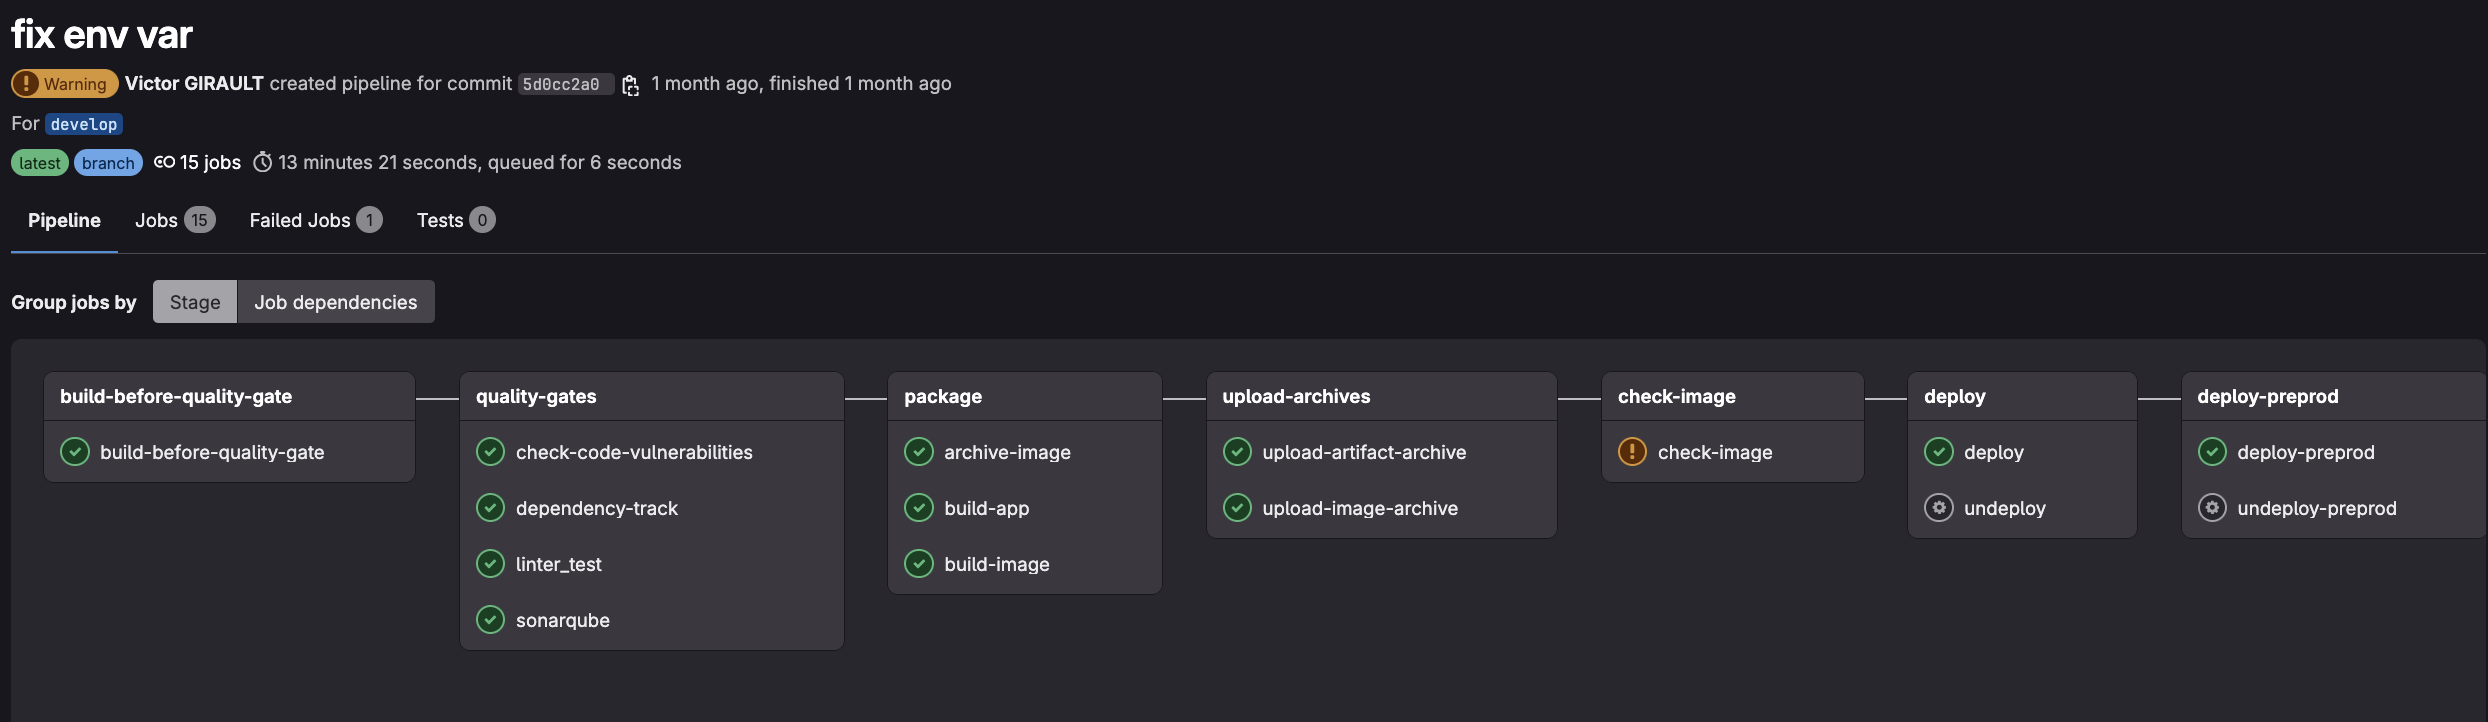
\includegraphics[width=\textwidth]{img/gitlab-ci-pipeline.png}
  \caption{Exemple de pipeline GitLab CI utilisée pour le déploiement de NijiSkills}
\end{figure}
\noindent
La pipeline CI impose l’exécution de plusieurs jobs obligatoires avant toute mise en production. Parmi ces étapes, on retrouve la vérification des tests unitaires et d’intégration, l’analyse du code via un linter pour assurer le respect des conventions de développement, ainsi que la vérification des dépendances afin de prévenir l’introduction de vulnérabilités ou d’incompatibilités. Ce processus rigoureux permet de détecter rapidement les éventuelles erreurs et d’assurer la stabilité de l’application à chaque modification du code.
\\
Une fois ces vérifications validées, la pipeline procède à la construction et au déploiement d’un ou plusieurs conteneurs Docker, selon la structure du projet. Ces conteneurs sont ensuite déployés sur Google Cloud Platform (GCP), où une forge dédiée héberge les projets en cours de développement. Cette infrastructure cloud offre une grande flexibilité et facilite la gestion des environnements de test et de préproduction.
\\
Pour les environnements de production, le processus de déploiement diffère afin de répondre à des exigences accrues en matière de sécurité, de disponibilité et de conformité. Des contrôles supplémentaires sont généralement appliqués, et le déploiement peut nécessiter des validations manuelles ou des étapes spécifiques propres à l’environnement de production. Cette distinction garantit que seules les versions les plus stables et sécurisées de l’application sont accessibles aux utilisateurs finaux.
\subsubsection{Sécurité et conformité}
La sécurité et la conformité ont été des axes majeurs dans la conception et le développement de NijiSkills. L’accès à l’application est strictement réservé aux collaborateurs de Niji grâce à la mise en place d’une authentification SSO (Single Sign-On) via Microsoft. Ce mécanisme d’authentification centralisée permet de garantir que seuls les utilisateurs disposant d’un compte professionnel Niji peuvent accéder à la plateforme. NijiSkills s'appuie sur l’infrastructure sécurisée de Microsoft Azure Active Directory. Cette dernière bénéficie d’un niveau de sécurité élevé pour la gestion des identités et des accès, tout en offrant une expérience utilisateur fluide et sans multiplication des mots de passe.
\\\\
Concernant la gestion des données, une attention particulière a été portée à la protection de la vie privée et à la minimisation des informations stockées. Aucune donnée personnelle sensible n’est enregistrée ou exploitée par NijiSkills: seule l’adresse e-mail professionnelle, indispensable à l’authentification et à l’identification des utilisateurs, est conservée en base de données. Ce choix délibéré de ne pas stocker d’autres informations personnelles permet de limiter les risques liés à la gestion des données et de se conformer aux principes de la réglementation sur la protection des données (RGPD). Ainsi, l’application s’inscrit dans une démarche responsable, en ne collectant que le strict nécessaire au bon fonctionnement du service.
\\\\
La sécurité du code et la robustesse de l’application sont également assurées par une pipeline d’intégration continue (CI) rigoureuse. Avant chaque mise en production, plusieurs jobs automatisés sont exécutés afin de garantir la qualité et la sécurité du code. Un linter analyse l’ensemble du code source pour vérifier le respect des conventions de développement et détecter d’éventuelles erreurs ou incohérences. Par ailleurs, l’outil DependencyTrack est utilisé pour analyser les dépendances du projet et s’assurer qu’aucune vulnérabilité connue n’est présente dans les bibliothèques utilisées. Ce processus de vérification systématique permet de prévenir l’introduction de failles de sécurité et de garantir que seules des versions stables et sûres de l’application sont déployées. L’ensemble de ces mesures contribue à offrir une solution fiable, sécurisée et conforme aux exigences actuelles en matière de développement logiciel.
\\\\
En complément de l’authentification SSO, l’accès à l’application NijiSkills est restreint au réseau interne de Niji. Cela signifie que l’application n’est accessible qu’aux collaborateurs connectés au réseau de l’entreprise, soit depuis les locaux de Niji, soit via un VPN sécurisé. Cette mesure supplémentaire permet de renforcer la sécurité en limitant l’exposition de l’application à l’extérieur et en réduisant les risques d’accès non autorisé. Ainsi, même en possession d’identifiants valides, un utilisateur ne pourra pas accéder à NijiSkills en dehors du périmètre réseau défini par l’entreprise.
\subsection{Fonctionnalités développées}
Dans cette section, je vais présenter en détail les principales fonctionnalités développées pour l’application NijiSkills. Pour chacune d’elles, j’expliquerai leur utilité, leur rôle dans l’application ainsi que les choix techniques et méthodologiques qui ont guidé leur mise en œuvre. Cette présentation permettra de mieux comprendre comment l’application a été conçue pour répondre aux besoins identifiés et les solutions apportées aux différents défis rencontrés lors du développement.
\subsubsection{Création et visualisation des thématiques}
Comme mentionné précédemment, l'une des principales fonctionnalités de NijiSkills est la création et la visualisation des thématiques. Chaque thématique représente un ensemble de compétences regroupées par domaine, permettant aux collaborateurs de mieux appréhender les compétences à acquérir pour progresser dans leur carrière. La visualisation se fait sous forme de "carte" interactive, où chaque compétence est représentée par un nœud, et les liens entre les compétences sont matérialisés par des flèches. Cette approche graphique facilite la compréhension des relations entre les différentes compétences et permet aux utilisateurs de naviguer aisément dans leur parcours de formation.
\\\\
Pour réaliser cette partie de l'application, j'ai utilisé la bibliothèque ReactFlow. En fouillant dans le repository public de roadmap.sh, j'ai remarqué que c'était la bibliothèque qu'ils utilisaient pour l'éditeur et la visualisation des thématiques. J'ai alors décidé de l'utiliser aussi pour NijiSkills car le but de ce projet était de se rapprocher le plus possible du fonctionnement global de roadmap.sh, tout en l'adaptant aux besoins spécifiques de Niji.
\\\\
ReactFlow est une librairie React qui permet de créer des graphes interactifs et dynamiques, avec la possibilité de personnaliser les nœuds, les liens et les interactions. Grâce à cette bibliothèque, j'ai pu implémenter une interface utilisateur intuitive et réactive, permettant aux collaborateurs de visualiser facilement leurs compétences et de naviguer entre les différentes thématiques.

\begin{figure}[H]
  \centering
  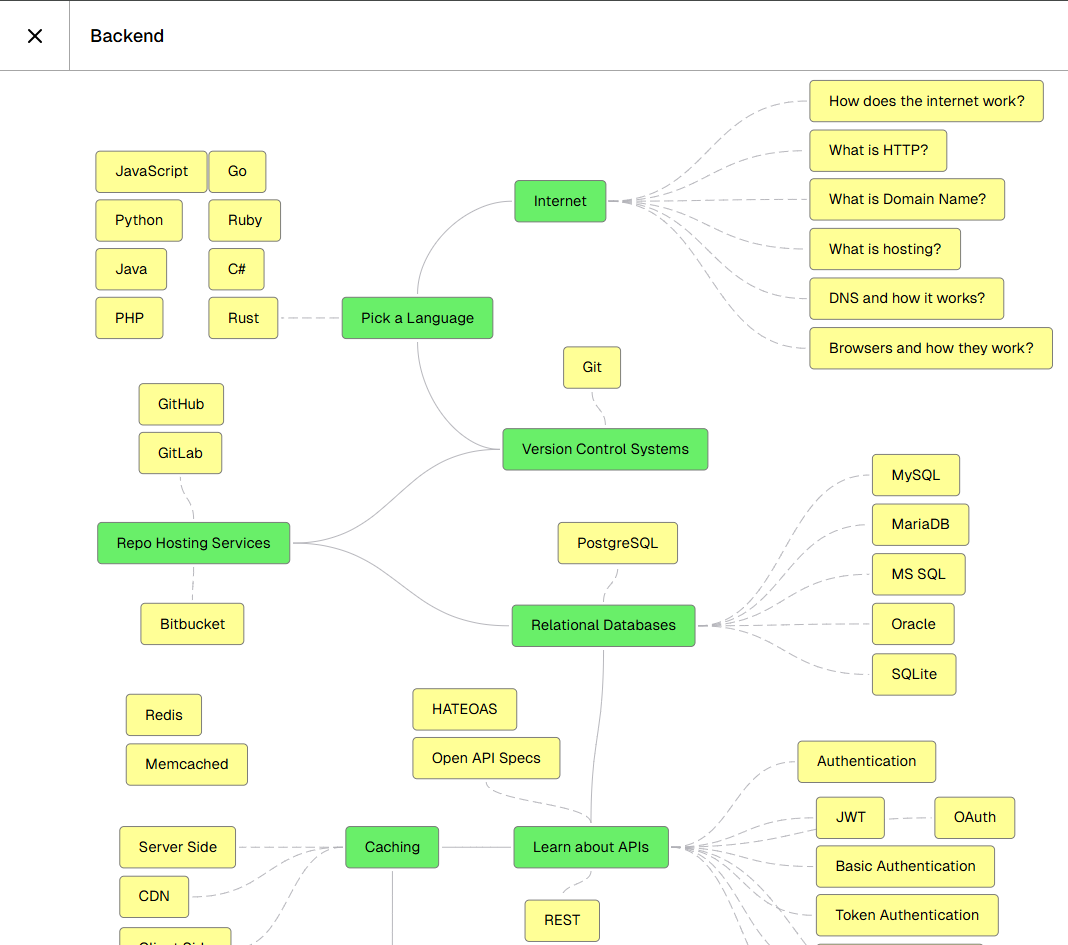
\includegraphics[width=0.75\textwidth]{img/nijiskills-view.png}
  \caption{Exemple de visualisation d'une thématique dans NijiSkills}
\end{figure}

La bibliothèque ReactFlow est plutôt simple à prendre en main, et permet de créer des graphes intéractifs de manière rapide et efficace. Il suffit simplement d'ajouter un composant \texttt{ReactFlow} dans le code, et de lui passer en props les nœuds et les liens à afficher. Voici à quoi pourrait ressembler le code pour créer un graphe basique avec ReactFlow :
\begin{figure}[H]
  \centering
  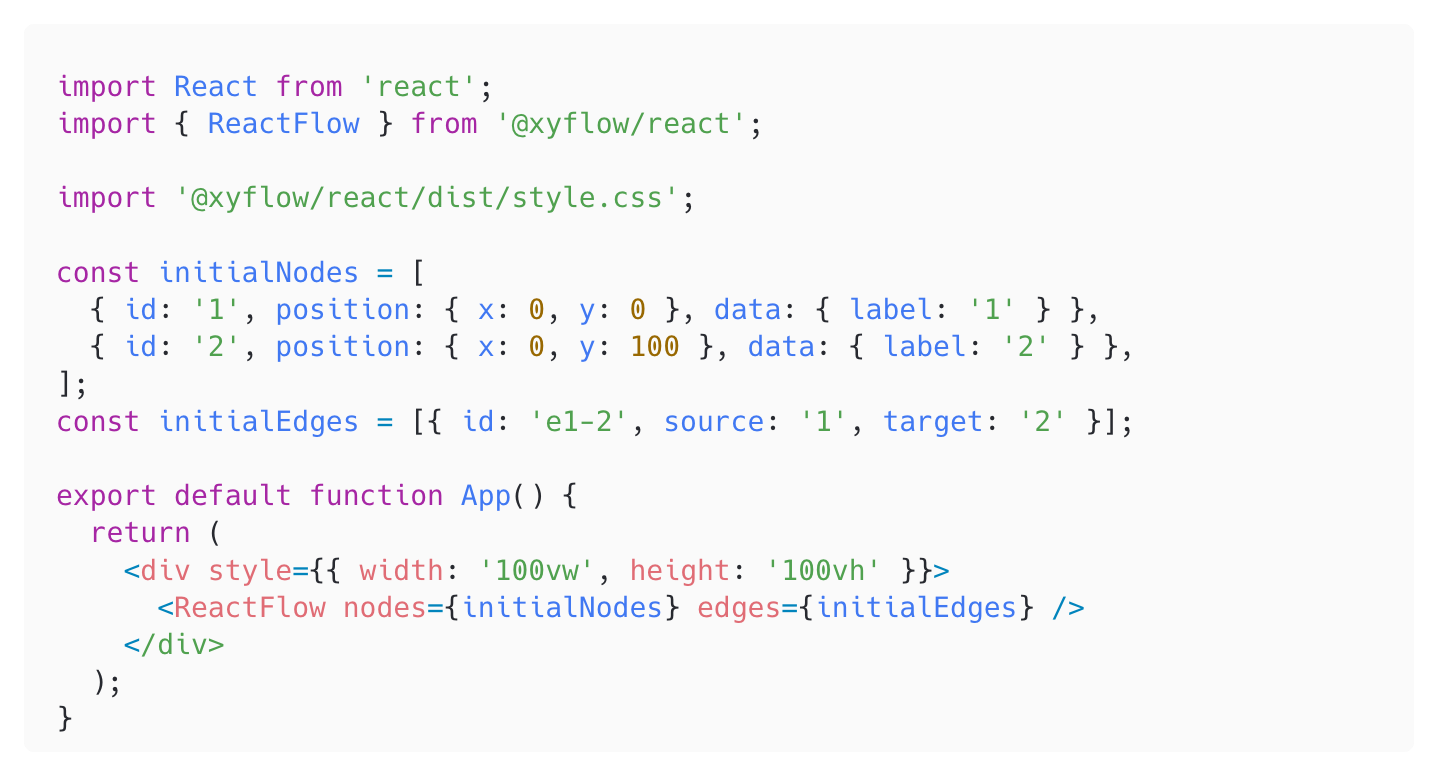
\includegraphics[width=0.80\textwidth]{img/reactflow-code.png}
  \caption{Exemple basique de création d'un graphe avec ReactFlow}
\end{figure}
\noindent
Mais pour avoir une version plus avancée qui corresponde à ce que l'on veut pour NijiSkills, il faut ajouter quelques options supplémentaires. Dans notre cas, il faut alors créer des noeuds personnalisés afin de distinguer les compétences primaires et les compétences secondaires. Les compétences primaires sont les compétences principales et indispensables à avoir pour continuer l'apprentissage d'une thématique, tandis que les compétences secondaires sont des compétences qui permettent d'approfondir les compétences primaires, mais qui ne sont pas indispensables pour continuer l'apprentissage de la thématique.
\\\\
Dans un second temps, il a fallu implémenter les régles de connexion entre les différents noeuds. Ces règles ont été définies dans la documentation utilisateur donnée aux testeurs, et permettent de définir comment peuvent être reliées les compétences. Les règles de connexion ont été définies comme suit :
\begin{quote}
  \begin{itshape}
    "La compétence principale (celle qui apparait obligatoirement et automatiquement à la création de la thématique et qui ne peut pas être supprimée) ne peut être reliée qu’à une seule autre compétence principale. Elle constitue le début du parcours de la thématique.
    \\\\
    Une compétence primaire ne peut être reliée qu’à deux autre compétence principale maximum: la compétence précédente et la compétence suivante dans le parcours de la thématique.
    \\\\
    Une compétence secondaire ne peut être reliée qu’à une et une seule compétence primaire. Plusieurs compétences secondaires peuvent être reliées à une même compétence primaire."
  \end{itshape}
\end{quote}
\vspace{0.5cm}
\noindent
Ces règles permettent de garantir une structure cohérente et logique des thématiques, en évitant les connexions illogiques ou redondantes entre les compétences. Elles assurent également que chaque thématique a un point de départ clair (la compétence principale) et un parcours défini, facilitant ainsi la navigation et l'apprentissage pour les utilisateurs.

\subsubsection{Gestion des versions des thématiques}
Pour répondre au besoin d’historiser les évolutions des thématiques et de permettre la gestion de plusieurs versions en parallèle, j’ai mis en place un système de versionning basé sur une table intermédiaire en base de données. Cette table fait le lien entre les thématiques, leurs versions et les compétences qui les composent, en stockant pour chaque version la liste des compétences et leur organisation (liens, types, etc.).
\begin{figure}[H]
  \centering
  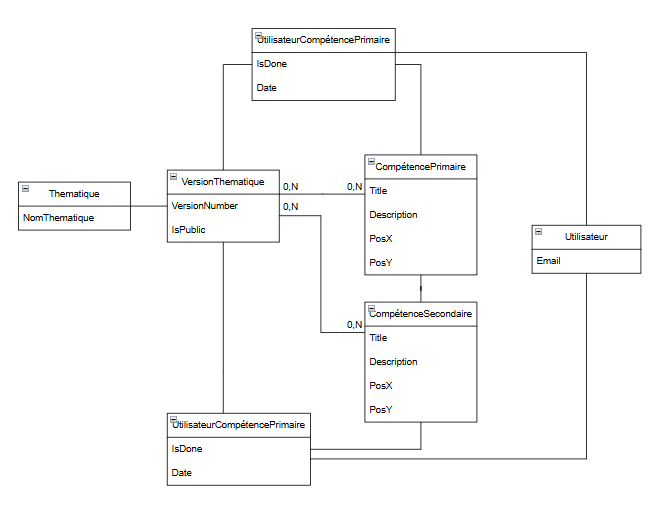
\includegraphics[width=0.85\textwidth]{img/bdd-version.png}
  \caption{Structure de la table intermédiaire pour le versionning des thématiques}
\end{figure}
Le principe de "copy-on-write" s’applique ici au niveau des compétences : une compétence est partagée entre plusieurs versions tant qu’elle n’est pas modifiée dans l'une d'elles. Lorsqu’une modification est apportée à une compétence dans une version donnée, une nouvelle copie de cette compétence est créée spécifiquement pour cette version, tandis que les autres versions continuent d’utiliser l’ancienne. Ainsi, seules les compétences modifiées sont dupliquées, ce qui optimise le stockage et garantit que chaque version reste figée dans le temps. Ce mécanisme permet de conserver l’historique des évolutions sans écraser les données existantes, et de restaurer facilement une version antérieure si besoin.
\\\\
La gestion des versions actives est également un point clé du système. À tout moment, une seule version d’une thématique est considérée comme "active" et visible par les utilisateurs. Les administrateurs disposent d’une interface leur permettant de sélectionner la version à activer parmi l’ensemble des versions existantes. Lorsqu’une nouvelle version est créée, elle n’est pas automatiquement activée : cela permet de préparer des évolutions en avance, de les tester ou de les valider avant de les rendre accessibles à tous. Ce mécanisme offre une grande flexibilité dans la gestion des évolutions, tout en assurant la stabilité de l’expérience utilisateur.
\begin{figure}[H]
    \centering
    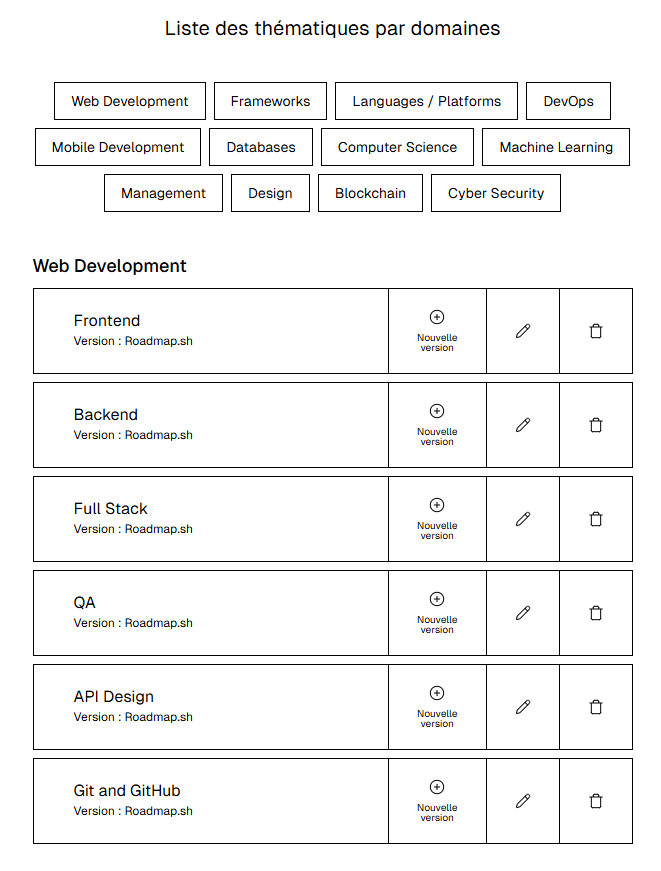
\includegraphics[width=0.65\textwidth]{img/listing-version.png} 
    \caption{Page de listing des thématiques avec les versions}
\end{figure}
En résumé, le versionning des thématiques repose sur une architecture de données adaptée (table intermédiaire), l’utilisation du "copy-on-write" au niveau des compétences pour garantir la non-destruction des versions précédentes, et un système de gestion des versions actives pour contrôler la visibilité des évolutions. Cette organisation assure à la fois la traçabilité, la sécurité et la flexibilité dans la gestion des thématiques au sein de NijiSkills.
\subsubsection{Panneau d'administration}
Le panneau d'administration de NijiSkills permet aux administrateurs de gérer les relations de management entre les collaborateurs, de gérer les domaines ainsi que de choisir la version active d'une thématique, c'est-à-dire la version qui sera visible par les utilisateurs. Les thématiques, elles, sont gérées par les administrateurs directement via la page de listing des thématiques.
\begin{figure}[H]
    \centering
    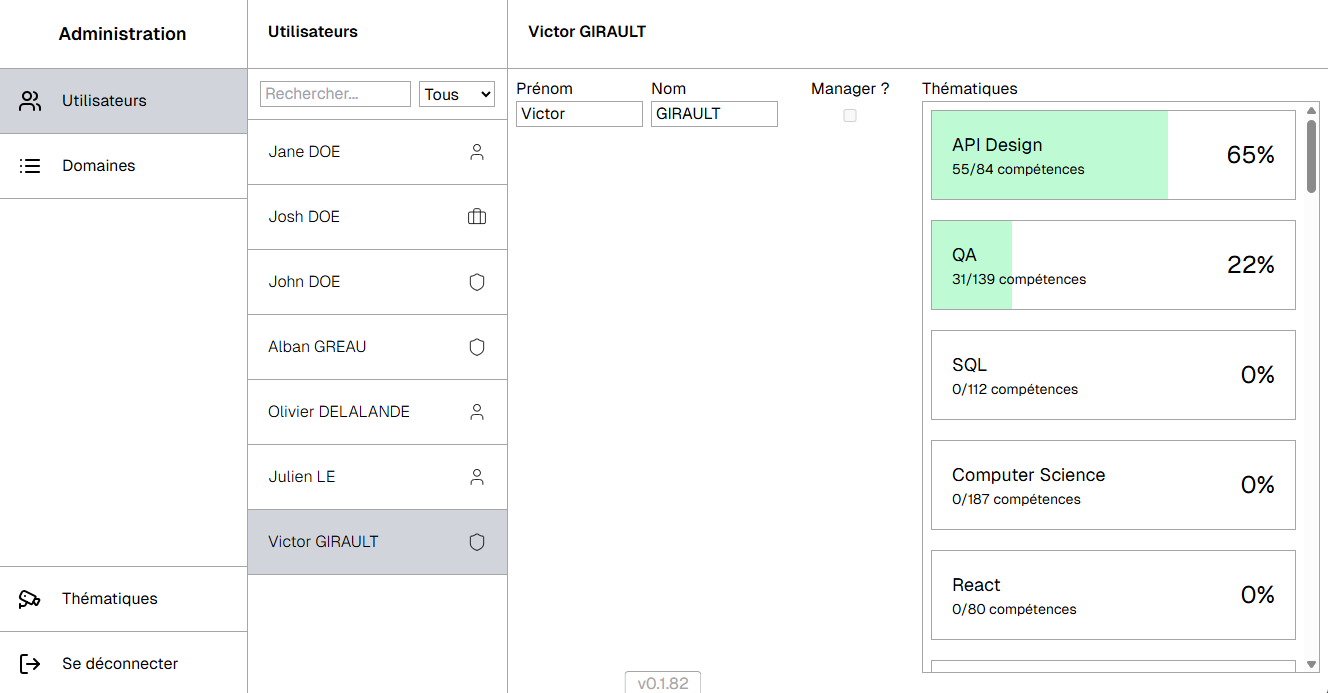
\includegraphics[width=0.85\textwidth]{img/admin-user.png} 
    \caption{Panneau d'administration des utilisateurs de NijiSkills}
\end{figure}

\begin{figure}[H]
    \centering
    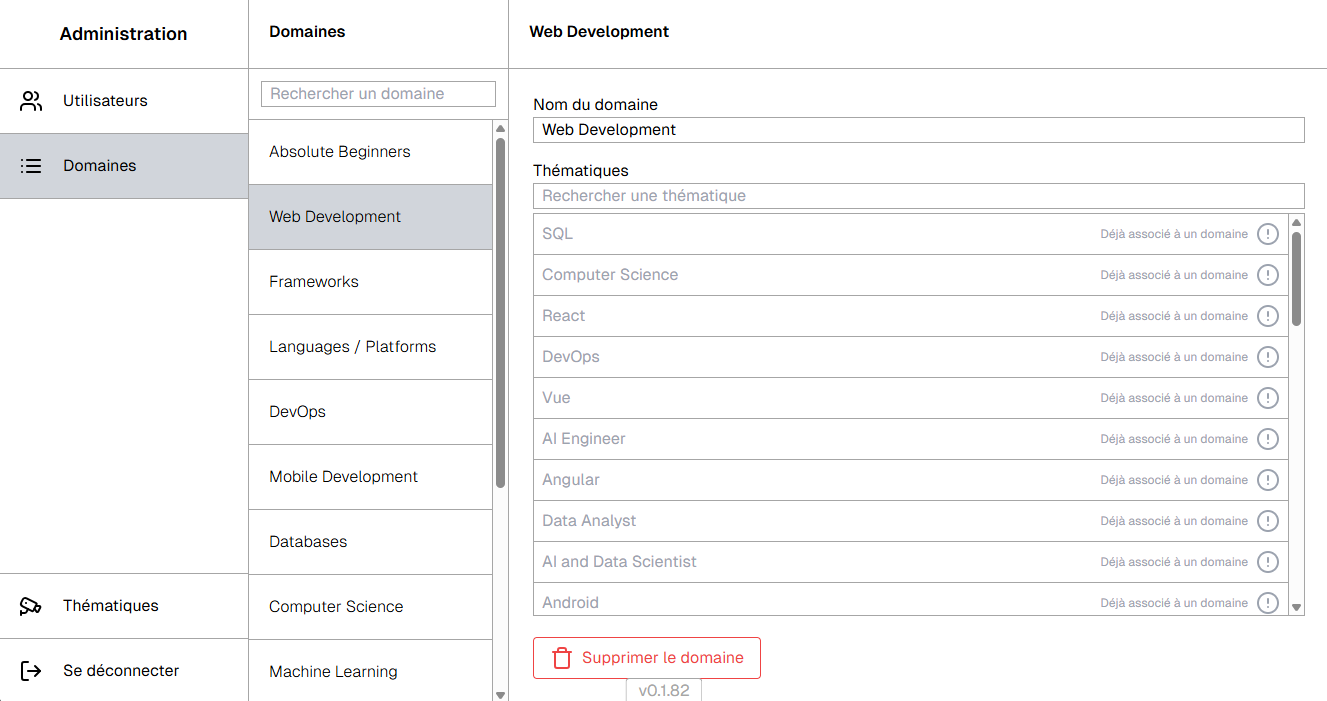
\includegraphics[width=0.85\textwidth]{img/admin-domain.png}
    \caption{Panneau d'administration des domaines de NijiSkills}
\end{figure}

\begin{figure}[H]
    \centering
    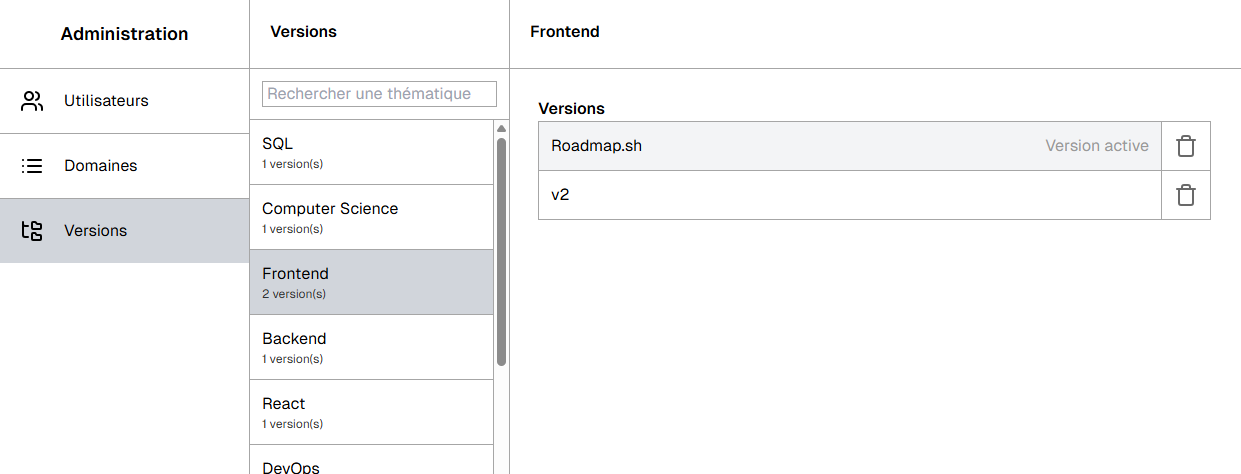
\includegraphics[width=0.85\textwidth]{img/admin-version.png}
    \caption{Panneau d'administration des versions de NijiSkills}
\end{figure}
Ces pages qui font office de "backoffice" ne sont accessibles que par les administrateurs. Les utilisateurs avec le rôle manager ont accès aussi à un panneau de gestion des utilisateurs qu'ils peuvent gérer, mais ils n'ont pas accès au panneau d'administration complet. Ils peuvent seulement voir la progression des utilisateurs qu'ils gèrent dans les différentes thématiques, ainsi que les compétences qu'ils ont validées ou non.

\subsubsection{Importation et exportation des thématiques}
Un élément important de l'application NijiSkills est la possibilité d'importer et d'exporter des thématiques au format JSON. Ces fonctionnalité servent, d'un côté, à garder une trace des thématiques créées avec les compétences, les liens et les différents utilisateurs qui aurait validé des compétences dans ces thématiques. D'un autre côté, elle permet aussi de partager des thématiques entre différents utilisateurs, ou de les exporter pour les utiliser dans d'autres applications. D'un autre côté, l'importation permet de récupérer des thématiques, notamment auxprès du site roadmap.sh, et de les proposer sur NijiSkills.
\\\\
Plusieurs fonctions ont alors été créées :
\paragraph{Importation des roadmaps officielles de roadmap.sh\\}
La fonction d'importation des roadmaps officielles de roadmap.sh permet de récupérer automatiquement les parcours de compétences créés et maintenus par l'équipe de roadmap.sh, considérés comme "officiels". Ces roadmaps sont accessibles via l'API publique du site, qui fournit un fichier JSON décrivant la structure de chaque roadmap (domaines, thématiques, compétences, liens, etc.).
\\\\
La fonction d'importation traduit ce JSON en thématiques et compétences compatibles avec le modèle de données de NijiSkills. Elle effectue un mapping entre les structures de roadmap.sh et celles utilisées dans l'application, en créant les thématiques correspondantes, en important les compétences et en reconstituant les liens entre elles.
\\\\
Enfin, la fonction classe automatiquement les thématiques importées par domaines, afin de conserver l'organisation logique proposée par roadmap.sh et de faciliter la navigation pour les utilisateurs de NijiSkills.
\paragraph{Importation d'une roadmap via son url roadmap.sh\\}
La fonction d'importation d'une roadmap via son URL roadmap.sh permet à tout utilisateur de NijiSkills d'importer une roadmap personnalisée, qu'elle soit publique ou privée, directement depuis la plateforme roadmap.sh. En effet, roadmap.sh offre à ses utilisateurs la possibilité de créer leurs propres roadmaps, qui peuvent être rendues publiques et partagées avec la communauté, ou bien rester privées et accessibles uniquement à leur créateur. Cette fonctionnalité d'importation fonctionne de manière similaire à l'importation des roadmaps officielles : il suffit de fournir l'URL de la roadmap souhaitée pour que NijiSkills récupère sa structure, ses compétences et ses liens, puis l'intègre dans l'application.
\\\\
Dans le cas où la roadmap à importer est privée, il est nécessaire de fournir un token d'authentification personnel généré sur roadmap.sh. Ce token permet à NijiSkills d'accéder aux données privées de l'utilisateur et de récupérer correctement la roadmap concernée. Sans ce token, seules les roadmaps publiques peuvent être importées. Cette approche garantit la sécurité et la confidentialité des données tout en offrant une grande flexibilité aux utilisateurs souhaitant exploiter leurs propres parcours de compétences au sein de NijiSkills.
\paragraph{Importation et exportation d'une roadmap via un fichier JSON\\}
Enfin, la fonction d'importation et d'exportation d'une roadmap via un fichier JSON permet aux administrateurs de NijiSkills de sauvegarder les thématiques et compétences sous forme de fichier JSON et de les réinsérer dans l'application. Ces fonctionnalités sont particulièrement utile pour conserver une copie locale des thématiques créées.
\subsection{Défis techniques rencontrés}
\subsubsection{Optimisation des performances}
L’une des principales difficultés rencontrées lors du développement de NijiSkills a été la gestion des performances du canvas interactif, rendu possible grâce à la bibliothèque ReactFlow. Cette librairie permet de manipuler dynamiquement un grand nombre de nœuds (représentant ici les compétences) et de liens entre eux, offrant une visualisation graphique intuitive des thématiques. Cependant, certaines thématiques peuvent contenir plusieurs dizaines, voire une centaine de compétences, chacune reliée à d’autres par des liens complexes. Cette densité d’informations peut rapidement entraîner un ralentissement notable de l’application, surtout lors du déplacement ou de la modification de nœuds, rendant l’expérience utilisateur moins fluide.
\\\\
Pour mieux comprendre les limites de ReactFlow, un stress test disponible sur le site officiel de la bibliothèque a été utilisé. Ce test démontre qu’il est possible d’afficher et de manipuler plusieurs centaines de nœuds sur un même canvas, à condition d’optimiser certains paramètres et de limiter les opérations coûteuses en ressources. Cela a permis d’identifier les axes d’amélioration nécessaires pour garantir de bonnes performances, même avec des thématiques très volumineuses.

\begin{figure}[H]
  \centering
  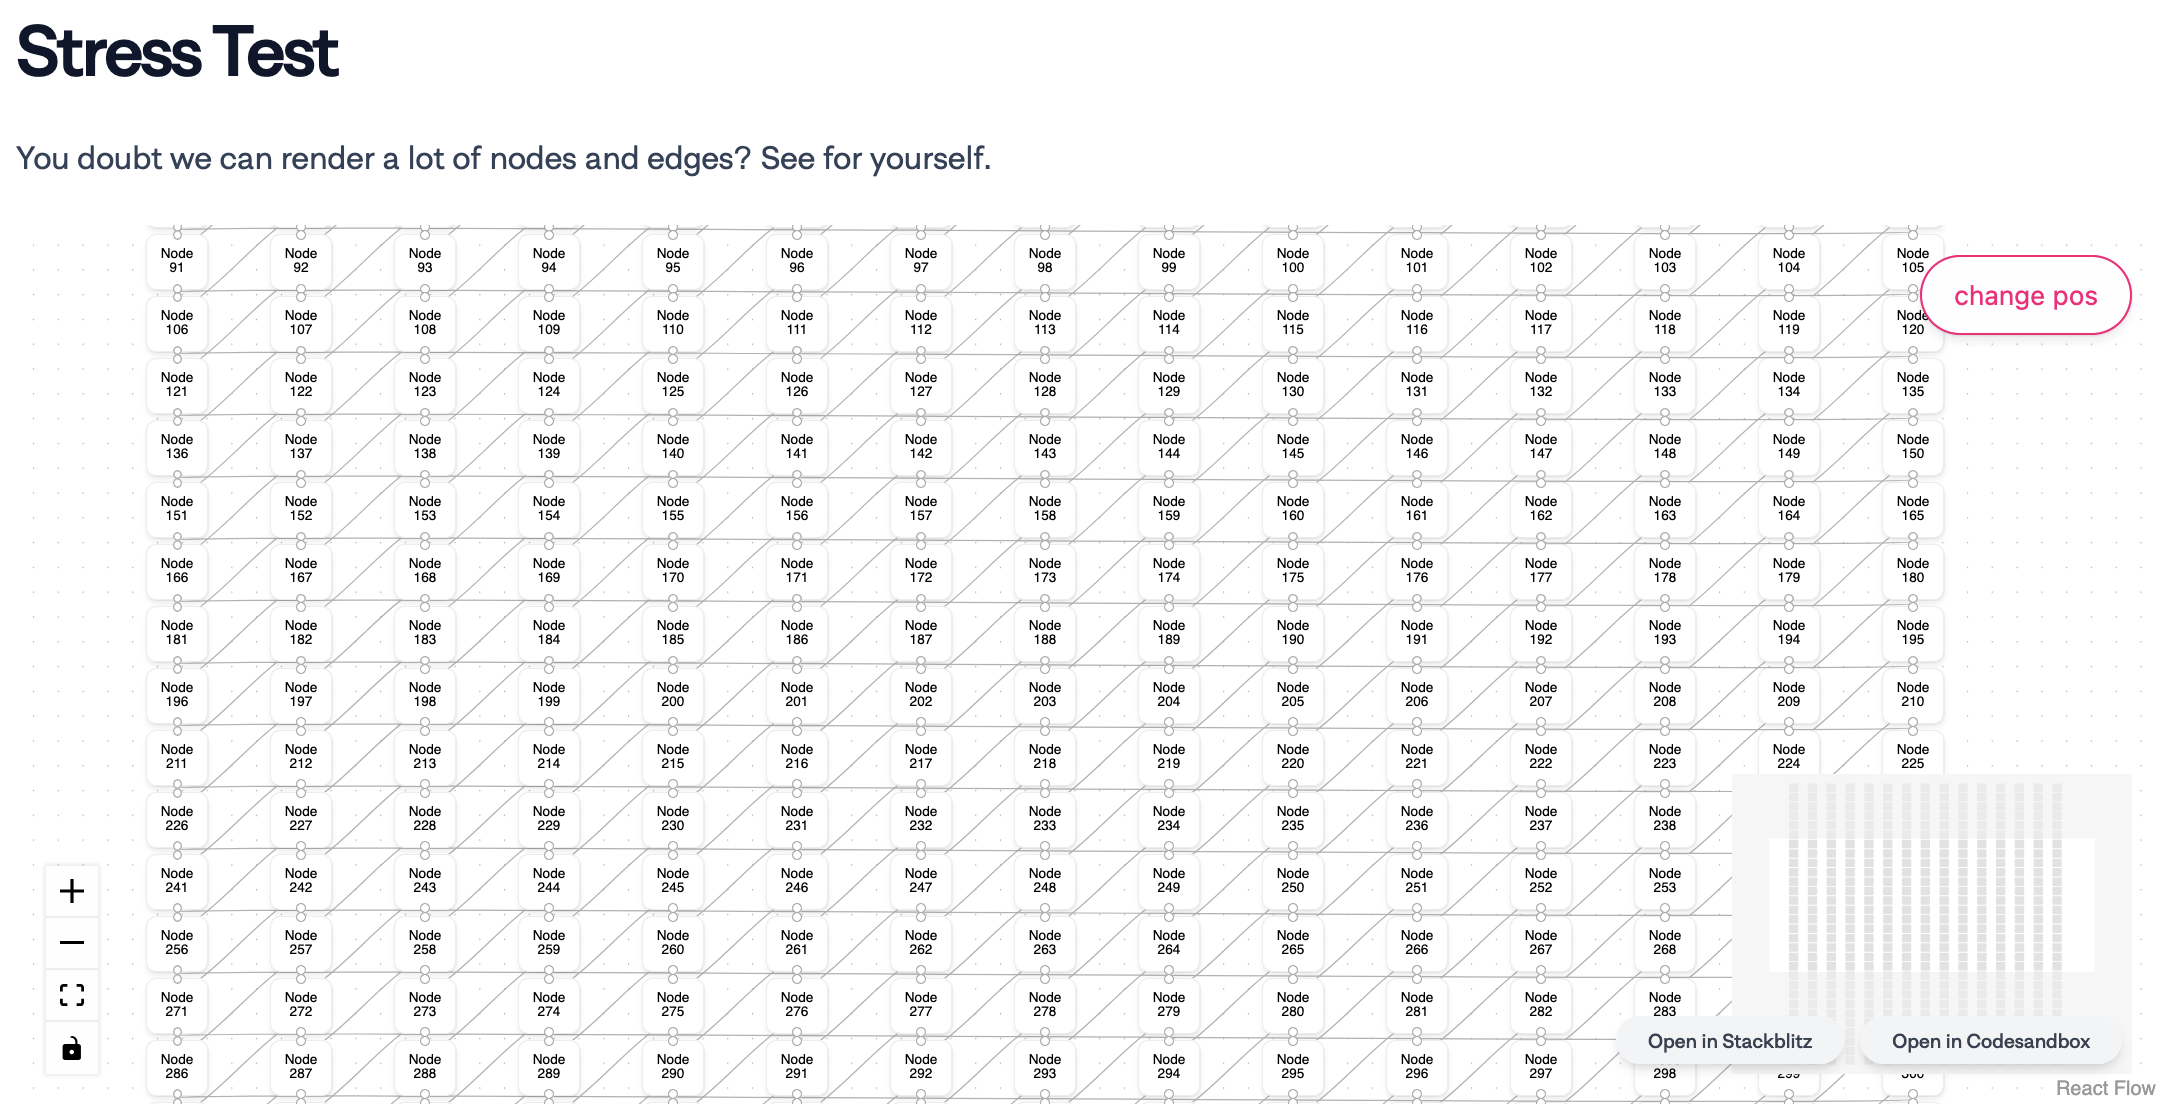
\includegraphics[width=0.85\textwidth]{img/stress-test.png}
  \caption{Stress test de ReactFlow affichant plusieurs centaines de nœuds}
\end{figure}
\noindent
Plusieurs optimisations ont donc été mises en place dans l’application. Tout d’abord, l’option de rendu conditionnel des nœuds a été activée : seuls les nœuds visibles à l’écran sont effectivement rendus et calculés par ReactFlow, tandis que ceux situés en dehors du champ de vision sont temporairement ignorés. Cette approche permet de réduire significativement la charge de calcul lors du rendu du canvas, en évitant de traiter inutilement des éléments invisibles pour l’utilisateur.
\\\\
Ensuite, la gestion de la sauvegarde automatique des modifications a été revue. Initialement, chaque modification sur le canvas (déplacement, ajout ou suppression de nœud) déclenchait une sauvegarde immédiate, ce qui pouvait saturer le serveur et ralentir l’interface. Pour remédier à cela, une fonction de sauvegarde « debounce » a été implémentée : les sauvegardes ne sont effectuées qu’après un court délai d’inactivité, ce qui permet de regrouper plusieurs modifications successives en une seule opération. Cette technique allège considérablement la charge sur le backend et améliore la réactivité globale de l’application.
\\\\
Grâce à ces ajustements, il a été possible d’assurer une expérience utilisateur fluide, même lors de la manipulation de thématiques complexes et très denses en compétences.
\subsubsection{Évolutions des besoins}
Au fil du développement, les besoins ont fortement évolué, entraînant de nombreuses demandes de nouvelles fonctionnalités. Tout d'abord, il est important de noter que le repository public de \texttt{roadmap.sh} ne contient pas le code source de l'éditeur ni du visionneur de thématique. Cette absence a nécessité de recréer entièrement ces modules, ce qui a représenté un travail conséquent pour garantir une expérience utilisateur cohérente et adaptée aux attentes.
\\\\
Par la suite, la demande de création de versions pour les thématiques a profondément bouleversé l'organisation des données dans la base de données ainsi que la structure de l'API. Il a fallu repenser la manière dont les thématiques étaient stockées, historisées et exposées, afin de permettre la gestion simultanée de plusieurs versions et d'assurer la compatibilité ascendante. Cette évolution a impliqué des modifications majeures tant au niveau du backend que du frontend, rendant l'architecture initiale obsolète face à ces nouveaux besoins.
\subsubsection{Propreté du code}
Un autre défi rencontré lors du développement de l’application a été de maintenir un code propre et bien structuré, tout en découvrant de nouveaux frameworks et en apprenant à coder « sur le tas ». Le fait de devoir produire une application finale tout en se formant à de nouveaux outils a rendu difficile l’adoption immédiate des meilleures pratiques de structuration et d’organisation du code. Les choix techniques ont souvent évolué au fil de l’apprentissage, ce qui a nécessité plusieurs phases de refactoring \footnote{Retravailler le code pour améliorer sa propreté sans toucher aux fonctionnalités} et de nettoyage du code au cours du projet. Il n’a donc pas toujours été évident de concilier apprentissage, expérimentation et production d’un code irréprochable dès les premières itérations.
\\\\
Pour répondre à cette problématique, plusieurs outils et pratiques ont été mis en place afin d’améliorer la qualité du code. L’intégration de SonarQube dans le processus de développement a permis d’identifier et de corriger de nombreux problèmes courants, tels que l’imbrication excessive de structures conditionnelles (\texttt{if}, \texttt{else}), la présence de fonctions trop volumineuses, ou encore les variables inutilisées ou non typées. SonarQube a ainsi encouragé le découpage du code en sous-fonctions plus petites et spécialisées, favorisant la lisibilité et la réutilisabilité. En complément, la mise en place d’un linter (ESLint) a automatisé le respect des conventions de codage, uniformisé le style du code et facilité la détection des erreurs de syntaxe ou de typage. L’association de SonarQube et du linter a donc permis d’instaurer une discipline de développement rigoureuse, tout en facilitant la détection et la correction des erreurs dès les premières phases du projet.

\subsection{Tests et validation}
\subsubsection{Tests unitaires}
Des tests unitaires ont été mis en place à l’aide du framework Jest afin de garantir la fiabilité et la robustesse de l’application. Chaque fichier contenant de la logique métier ou des fonctions critiques est accompagné de tests unitaires dédiés, permettant de vérifier le bon fonctionnement de chaque composant de manière isolée. Cette approche assure que les différentes parties de l’application réagissent correctement face à des cas d’utilisation variés, tout en facilitant la détection rapide d’éventuelles régressions lors de l’ajout de nouvelles fonctionnalités.
\\\\
L’exécution de la suite de tests unitaires est intégrée directement dans la pipeline d’intégration et de déploiement continue (pipeline CI/CD) \footnote{Série d'étapes automatisée pour déployer une nouveller version d'un logiciel}. Ainsi, à chaque modification du code, l’ensemble des tests est automatiquement lancé. Si un seul test échoue, la pipeline est interrompue et le déploiement de l’application est bloqué. Ce mécanisme garantit que seules des versions validées et stables peuvent être mises en production, renforçant la qualité globale du projet.
\\\\
En complément, l’outil SonarQube est utilisé pour analyser la couverture des tests unitaires sur le code source. Il est possible d’imposer un seuil minimal de couverture, par exemple 60\%, afin de s’assurer qu’une part significative du code est effectivement testée. Si ce taux n’est pas atteint, la pipeline peut également être bloquée, obligeant les développeurs à ajouter les tests nécessaires avant de poursuivre le déploiement. Cette exigence contribue à maintenir un haut niveau de qualité et de fiabilité pour l’ensemble de l’application.
\begin{figure}[H]
  \centering
  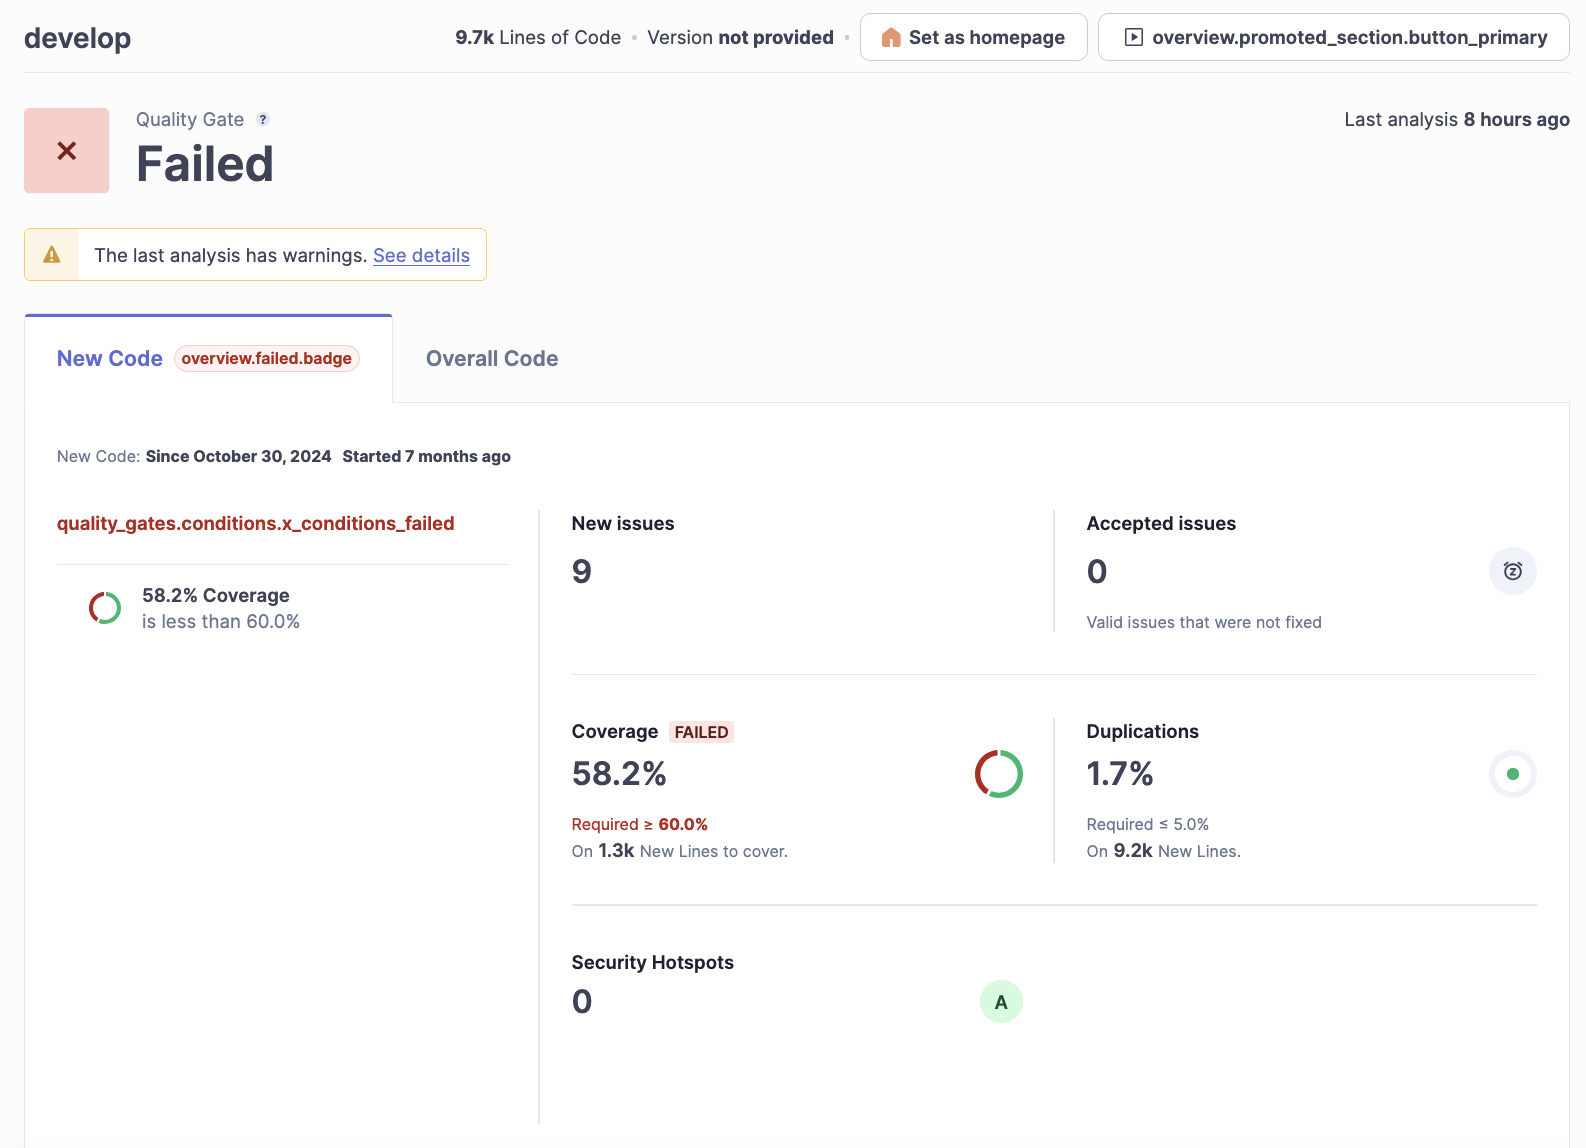
\includegraphics[width=0.85\textwidth]{img/sonarqube.png}
  \caption{Exemple de rapport SonarQube montrant la couverture des tests unitaires}
\end{figure}
\subsubsection{Tests End to End}
À la fin du mois de mai 2025, l’intégration de Playwright pour compléter la couverture des tests unitaires était en cours de réflexion au sein du projet NijiSkills. Cette démarche s’inscrit dans une volonté d’améliorer la qualité globale de l’application en ajoutant des tests end-to-end (E2E) automatisés, capables de valider le bon fonctionnement de l’ensemble des parcours utilisateurs. La réflexion autour de l’adoption de Playwright a été soutenue par Tanguy MICHEL, développeur au sein de l’équipe DSF à Rennes, qui suit de près l’évolution des fonctionnalités de Playwright et partage régulièrement ses retours d’expérience avec les autres membres de l’équipe. Grâce à sa veille technologique, Tanguy a pu mettre en avant les avantages de cet outil et encourager son adoption pour renforcer la stratégie de tests du projet.
\\\\
À ce jour, Playwright n’est pas encore intégré au sein de NijiSkills, mais il y a de fortes chances qu’il le soit prochainement. L’ajout de Playwright permettrait d’automatiser des scénarios de tests simulant le comportement réel des utilisateurs sur l’application, depuis la connexion jusqu’à la manipulation des différentes fonctionnalités. Playwright se distingue par sa capacité à piloter plusieurs navigateurs (Chromium, Firefox, WebKit) et à gérer des cas complexes, comme l’authentification SSO ou les interactions avec des éléments dynamiques du DOM. Il offre également des fonctionnalités avancées telles que la génération de rapports détaillés, la capture de screenshots et l’enregistrement de vidéos lors de l’exécution des tests, facilitant ainsi l’analyse des éventuels dysfonctionnements.
\\\\
En résumé, Playwright pourrait jouer un rôle clé dans l’amélioration de la fiabilité et de la robustesse de NijiSkills, en permettant de valider automatiquement les parcours critiques de l’application et en détectant rapidement les régressions lors des évolutions du code.
\subsubsection{Tests utilisateurs}
À ce stade du projet, des tests utilisateurs sont prévus mais n'ont pas encore été réalisés. Ces tests seront menés par un groupe de testeurs internes chez Niji. L'objectif de ces tests est de recueillir des retours concrets sur l'ergonomie, la facilité d'utilisation et la pertinence fonctionnelle de la solution développée. Ils permettront d'identifier d'éventuels points d'amélioration, de valider les choix techniques effectués et de s'assurer que le produit final répond bien aux besoins des utilisateurs finaux.

\newpage
\section{Retour d’expérience, prise de recul et conclusion}
\subsection{Compétences développées}
Dans cette section, je vais présenter les différentes compétences que j'ai pu développer au cours de ce projet, tant sur le plan technique que méthodologique et personnel. Je vais également expliquer comment ces compétences ont été mises en pratique dans le cadre du projet NijiSkills et comment elles pourront être utiles pour mes futurs projets professionnels.
\subsubsection{Compétences techniques}
Au cours de ce projet, j’ai pu approfondir mes connaissances sur le framework Next.js, en particulier sur la distinction et l’utilisation des composants client et serveur. Bien que je disposais déjà de bonnes bases en React, ce projet m’a permis de comprendre plus en détail les spécificités de Next.js, notamment l’optimisation des performances et de la sécurité grâce au rendu côté serveur (Server Components), ainsi que l’utilisation des composants client pour l’interactivité. J’ai ainsi amélioré ma capacité à structurer une application, à gérer le cycle de vie des données, à implémenter des appels API efficaces et à garantir une expérience utilisateur fluide et réactive.
\\\\
J’ai également acquis une expérience significative dans la mise en place de pipelines CI/CD avec GitLab. J’ai appris à configurer des pipelines automatisées pour assurer la qualité du code, l’exécution des tests unitaires, l’analyse statique avec des outils comme SonarQube, et le déploiement automatisé sur des environnements cloud. Cette compétence m’a permis de comprendre l’importance de l’automatisation dans le cycle de développement logiciel, de réduire les risques d’erreurs humaines et d’accélérer la livraison de nouvelles fonctionnalités.
\\\\
Enfin, le projet m’a permis de valider mes compétences en conteneurisation avec Docker. J’ai appris à créer et optimiser des images Docker pour l’application et ses dépendances, à gérer les volumes et les réseaux, et à orchestrer le déploiement sur différents environnements. Cette maîtrise de Docker m’a permis de garantir la portabilité de l’application, de faciliter la gestion des environnements de développement et de production, et d’assurer une meilleure reproductibilité des déploiements.
\subsubsection{Compétences méthodologiques}
Le fait d’avoir développé ce projet en grande partie en autonomie m’a permis de renforcer plusieurs compétences méthodologiques essentielles. J’ai appris à organiser et planifier mon travail de manière rigoureuse, en définissant moi-même les priorités et en adaptant la planification en fonction des imprévus ou des évolutions du projet.
\\\\
J’ai également développé ma capacité à m’auto-former et à faire de la veille technologique: face à des problématiques nouvelles, j’ai su rechercher, tester et comparer différentes solutions, tout en restant attentif aux bonnes pratiques du secteur. La nécessité de produire un code maintenable et de qualité m’a amené à instaurer des standards (tests, CI/CD, documentation) et à m’auto-évaluer régulièrement, en procédant à des phases de refactoring lorsque cela s’avérait nécessaire.
\\\\
Enfin, même en travaillant seul, j’ai appris à communiquer efficacement avec les intervenants ponctuels du projet, en formulant clairement mes besoins et en documentant mes avancées pour faciliter les échanges. Cette expérience m’a permis de gagner en autonomie, en rigueur et en capacité d’adaptation, des qualités indispensables pour mener à bien des projets complexes dans un environnement professionnel.
\subsubsection{Compétences personnelles}
Ce projet m’a permis de développer de nombreuses compétences personnelles. Travailler en autonomie m’a appris à faire preuve d’organisation, de rigueur et à gérer efficacement mon temps pour atteindre les objectifs fixés. 
\\\\
La nécessité de surmonter seul les difficultés rencontrées m’a permis de développer ma persévérance et ma capacité à trouver des solutions par moi-même notamment lors de la résolution de problèmes complexes ou face à des imprévus. J’ai également appris à m’adapter rapidement à de nouveaux outils et à des changements de priorités, ce qui a renforcé ma flexibilité et mon agilité.
\\\\
Enfin, cette expérience a stimulé ma curiosité et mon envie d’apprendre : j’ai su aller chercher l’information, me remettre en question et adopter une démarche d’amélioration continue, tant sur le plan technique que personnel.
\newpage
\subsection{Comparaison entre les entreprises de différentes tailles}
Dans cette section, je vais comparer mon expérience de stage chez Niji avec celle que j'ai pu avoir dans une petite entreprise. Je vais aborder les différences en termes d'environnement de travail, d'encadrement et d'autonomie, ainsi que l'organisation des projets.
\subsubsection{Environnement de travail}
Dans une grande entreprise comme Niji, l’environnement de travail se caractérise par une organisation structurée et des processus bien établis. Les locaux sont généralement modernes, spacieux et conçus pour accueillir un grand nombre de collaborateurs, avec des espaces dédiés à la collaboration, à la concentration ou à la détente. L’infrastructure informatique est souvent plus performante, avec des outils professionnels et des ressources partagées à grande échelle. Cependant, cette organisation peut parfois donner une impression d’anonymat, notamment lorsqu’on travaille seul sur un projet ou que l’on n’est pas intégré à une équipe existante. À l’inverse, dans une petite entreprise, l’ambiance est souvent plus conviviale et familiale, les échanges sont plus informels et la proximité avec les collègues favorise la cohésion et l’entraide au quotidien. Les espaces de travail sont généralement moins formalisés, mais la flexibilité et la rapidité de prise de décision sont souvent plus grandes.

\subsubsection{Encadrement et autonomie}
Le niveau d’encadrement diffère également entre grande et petite entreprise. Dans une structure comme Niji, l’encadrement est plus formalisé : il existe des processus de suivi, des points réguliers avec les chefs de projets ou managers, et des outils de gestion de projet qui permettent de suivre l’avancement et de remonter les difficultés. Cette organisation offre un cadre rassurant, mais peut parfois limiter l’autonomie dans la prise de décision. À l’inverse, dans une petite entreprise, l’encadrement est souvent plus souple et informel. On bénéficie d’une plus grande autonomie et d’une liberté d’initiative, mais cela implique aussi de savoir s’auto-organiser et de prendre des responsabilités rapidement. L’apprentissage se fait souvent « sur le tas », avec un accès direct aux dirigeants ou aux décideurs, ce qui peut accélérer la montée en compétences.

\subsubsection{Organisation des projets}
L’organisation des projets dans une grande entreprise repose sur des méthodes éprouvées (agilité, gestion de projet, documentation, outils collaboratifs) et une répartition claire des rôles. Les projets sont généralement plus structurés, avec des jalons, des revues régulières et une gestion des risques plus formalisée. Cela permet de garantir la qualité et la pérennité des livrables, mais peut parfois ralentir la prise de décision ou l’innovation à cause de la lourdeur des processus. Dans une petite entreprise, les projets sont souvent menés de façon plus agile et réactive, avec moins de formalisme et une communication directe entre les membres de l’équipe. Cette souplesse permet d’adapter rapidement les priorités, mais peut aussi entraîner un manque de documentation ou de suivi, et une dépendance plus forte à l’implication individuelle de chacun. Enfin, la diversité des missions dans une petite structure permet souvent de toucher à plusieurs aspects d’un projet, tandis que dans une grande entreprise, la spécialisation des rôles est plus marquée.

\subsection{Axes d’amélioration personnelle}
Dans cette section, je vais identifier les axes d'amélioration personnelle que j'ai pu identifier au cours de ce projet. Je vais aborder les points sur lesquels je pense pouvoir progresser, tant sur le plan technique que personnel, et comment je compte m'y prendre pour y parvenir.
\subsubsection{Choix techniques}
Avec le recul, je pense qu’il aurait été bénéfique de prendre davantage de temps pour réfléchir à l’architecture globale du projet avant de commencer à coder. Par exemple, l’organisation des fichiers aurait pu être plus structurée, ce qui aurait facilité la maintenance et la compréhension du code. De même, la conception des tables de la base de données aurait pu être mieux anticipée et refactorisée afin de simplifier leur traitement par la suite. Ces difficultés s’expliquent en partie par l’évolution constante du projet pendant son développement, les bases et les besoins n’étant pas totalement définis dès le départ.
\\\\
Concernant les choix des technologies, je pense qu'elles ont été globalement pertinentes, mais j’aurais pu approfondir certaines d’entre elles, notamment Next.js et ReactFlow. Par exemple, j’aurais pu explorer plus en détail les Server Components de Next.js pour optimiser encore davantage les performances de l’application. De même, une meilleure compréhension des capacités avancées de ReactFlow, en créant un projet d'entraînement par exemple, aurait permis d’implémenter des fonctionnalités plus complexes plus rapidement dès le début du projet.
\subsubsection{Gestion de projet}
J’aurais aussi pu aller plus loin dans l’exploitation des outils de gestion de projet, notamment en affinant le découpage des tâches et en planifiant plus précisément leur réalisation. Par exemple, au lieu de regrouper certaines fonctionnalités sous des tâches larges, il aurait été pertinent de les diviser en sous-tâches plus granulaires, ce qui aurait permis un suivi plus fin de l’avancement et une meilleure anticipation des difficultés potentielles. Cela m’aurait également aidé à mieux estimer le temps nécessaire pour chaque étape et à ajuster plus rapidement la planification en cas d’imprévus.
\\\\
De plus, j’aurais pu utiliser davantage les fonctionnalités avancées de Jira, telles que la gestion des dépendances entre tâches, la définition de jalons intermédiaires ou la programmation de rappels automatiques. Cela aurait permis d’avoir une vision encore plus claire de la progression du projet et de mieux prioriser les actions à mener. Enfin, une programmation plus rigoureuse des tâches dans le temps, avec des échéances intermédiaires, m’aurait aidé à structurer davantage mon travail et à limiter les périodes de flottement ou de surcharge.
\\\\
En résumé, une utilisation plus poussée des outils de gestion de projet, associée à un découpage plus fin et une programmation détaillée des tâches, aurait permis d’optimiser l’organisation du projet, d’améliorer la visibilité sur l’avancement et de gagner en efficacité tout au long du développement.
\subsubsection{Organisation personnelle}
Du coté de l'organisation personnelle, j'ai pu identifier plusieurs axes d'amélioration.
\\\\
Même si mon organisation personnelle n’était pas fondamentalement désordonnée, j’ai identifié plusieurs axes d’amélioration. J’aurais pu, par exemple, formaliser davantage mes routines de travail en définissant des plages horaires fixes pour certaines tâches (veille technologique, rédaction de documentation, revue de code). Mettre en place des to-do lists quotidiennes ou hebdomadaires plus détaillées m’aurait permis de mieux visualiser l’avancement et de prioriser efficacement les actions à mener. J’aurais aussi pu consacrer du temps régulier à la prise de recul, en planifiant des bilans intermédiaires pour ajuster mes méthodes si besoin. Enfin, mieux anticiper les périodes de forte charge ou de baisse de motivation, en adaptant mon planning ou en sollicitant plus tôt de l’aide, aurait contribué à une gestion du temps encore plus efficace et à limiter le stress lors des phases critiques du projet.
\\\\
Bien que ces axes d’amélioration n’aient pas eu d’impact majeur sur le projet, ils auraient permis de gagner en sérénité et en efficacité au quotidien. En intégrant ces bonnes pratiques dans ma routine de travail, je suis convaincu que je pourrai améliorer encore ma productivité et la qualité de mes livrables dans mes futurs projets professionnels.
\subsection{Impact du projet chez Niji}
Je vais maintenant présenter où en est le projet NijiSkills aujourd'hui et quelles sont les perspectives d'évolution envisagées pour l'avenir.
\subsubsection{Utilisation actuelle}
À l’heure actuelle, le projet NijiSkills est toujours en phase de développement actif. De nouvelles fonctionnalités sont régulièrement envisagées et des améliorations sont apportées en continu, que ce soit sur le plan technique ou fonctionnel. Malgré ce statut de projet en évolution, l’application est d’ores et déjà pleinement opérationnelle et utilisable par les collaborateurs de Niji. Toutes les fonctionnalités principales, telles que la gestion des thématiques, la visualisation des compétences, l’import/export de roadmaps ou encore l’administration des utilisateurs, sont en place et fonctionnent de manière fiable. La mise en place de la mise à jour des CVs des utilisateurs sur DoYouBuzz est encore en cours de développement, mais elle devrait être finalisée très prochainement.
L'application est destinée à être utilisée par les collaborateurs de Niji dans les mois qui arrivent.
\subsubsection{Perspectives d’évolution}
Plusieurs pistes d'évolutions ont déjà été réflechies pour le projet NijiSkills. Parmi celles-ci, on peut citer :
\begin{itemize}
  \item \textbf{Intégration de Playwright pour les tests end-to-end} : Comme mentionné précédemment, l’intégration de Playwright est envisagée pour automatiser les tests E2E et valider les parcours utilisateurs de manière plus exhaustive.
  \item \textbf{Amélioration de l’interface utilisateur} : Des retours d’expérience utilisateurs seront collectés pour identifier les points d’amélioration de l’ergonomie et de la navigation au sein de l’application. Des ajustements visuels et fonctionnels seront réalisés en conséquence par une équipe dédiée à l’expérience utilisateur (UX) chez Niji.
  \item \textbf{Ajout d'un serveur MCP} : Un serveur MCP (Model Control Protocol) pourrait être mis en place pour permettre aux IAs conversationnelles de Niji d'interagir directement avec NijiSkills. Cela permettrait de faciliter l'accès aux thématiques et compétences via des interfaces conversationnelles, rendant l'application plus accessible et intuitive pour les utilisateurs.
\end{itemize}
\noindent
\newline
Ces évolutions permettront de renforcer l’application, d’améliorer l’expérience utilisateur et de garantir la pérennité du projet dans le temps. L’objectif est de faire de NijiSkills un outil incontournable pour accompagner les collaborateurs dans leur montée en compétences et leur développement professionnel au sein de Niji.
\subsection{Perspectives professionnelles}
\subsubsection{Suite de parcours}
À l’issue de cette alternance, mon objectif principal est de poursuivre mon parcours professionnel dans le développement logiciel, idéalement au sein de Niji si une opportunité d’embauche se présente. L’environnement de travail, la diversité des projets et la culture d’entreprise correspondent à mes attentes et me motivent à continuer à évoluer dans ce cadre.
\\\\
Si cela n’est pas possible, je souhaite mettre à profit les compétences acquises lors de ce projet pour intégrer une équipe technique dynamique, que ce soit dans une ESN, une startup ou une entreprise du secteur numérique.
\\\\
Ce projet m’a également conforté dans une idée que j’avais avant de rejoindre Niji : m’orienter vers un langage plus typé, voire potentiellement orienté objet, afin d’avoir davantage de contrôle sur la structure de mes applications et d’éviter de partir dans toutes les directions comme cela peut arriver en JavaScript. L’utilisation de TypeScript m’a déjà permis de constater les bénéfices d’un typage plus strict, mais je souhaite approfondir cette démarche avec des langages comme Java, C\# ou même C++, pour gagner en rigueur et en maintenabilité.
\\\\
À moyen terme, j’ambitionne de me spécialiser dans les technologies modernes du web (Next.js, cloud, CI/CD) tout en continuant à développer mes compétences en gestion de projet et en encadrement d’équipe. Je suis convaincu que l’expérience acquise au sein de Niji, tant sur le plan technique que méthodologique, sera un atout précieux pour la suite de mon parcours professionnel.
\subsubsection{Réflexions sur le domaine d’activité}
Mon expérience au sein de Niji m’a permis de mieux appréhender les enjeux et les spécificités du secteur du numérique, et plus particulièrement des ESN. J’ai constaté à quel point ce domaine est en constante évolution : les technologies, les méthodes de travail et les attentes des clients changent rapidement, ce qui impose une veille technologique permanente et une grande capacité d’adaptation.
\\\\
L’innovation occupe une place centrale dans ce secteur : il est essentiel de tester de nouveaux outils, d’expérimenter des approches différentes et de se former en continu pour rester compétitif. J’ai également réalisé que, même dans un environnement très technique, les compétences humaines sont tout aussi importantes : la communication, la gestion de projet et l’autonomie sont indispensables pour mener à bien des projets complexes.
\\\\
Enfin, la transformation digitale des entreprises crée de nombreuses opportunités, mais aussi des défis importants, notamment en matière de sécurité, de gestion du changement et d’accompagnement des utilisateurs. Ce secteur est particulièrement stimulant pour les jeunes diplômés, à condition de rester curieux, motivé et prêt à se remettre en question en permanence.
\subsubsection{Apparté sur l'impact de l'intelligence artificielle dans le développement informatique}
L’intelligence artificielle (IA) occupe une place de plus en plus importante dans le secteur du développement informatique, notamment à travers l’émergence d’outils et d’environnements de développement intégrés (IDE) orientés IA. Durant ce projet, j’ai eu l’occasion d’expérimenter des IDE nouvelle génération comme Cursor ou Windsurf, qui intègrent nativement des assistants IA pour accompagner le développeur au quotidien. Ces outils proposent des fonctionnalités avancées telles que la génération automatique de code, la suggestion de corrections ou d’optimisations, l’explication de blocs de code complexes, ou encore la rédaction assistée de documentation technique.
\\\\\\
L’utilisation de ces IDE m’a permis de gagner en efficacité, de réduire le temps passé sur certaines tâches répétitives et d’améliorer la qualité du code produit. L’IA s’avère particulièrement utile pour accélérer la recherche de solutions à des problèmes techniques, générer des tests unitaires ou encore proposer des exemples d’implémentation adaptés au contexte du projet. Cette démocratisation des outils IA dans le développement ouvre de nouvelles perspectives, tant pour l’apprentissage que pour la productivité, et constitue un atout majeur pour rester compétitif dans un secteur en constante évolution.
\subsection{Conclusion générale}
Ce rapport conclut une année d’alternance très formatrice, marquée par la découverte de nouveaux outils, de nouvelles méthodes de travail et de nombreux défis. Le développement de NijiSkills m’a permis de mettre en pratique mes connaissances, d’en acquérir de nouvelles et de mieux comprendre le fonctionnement d’un projet informatique dans une grande entreprise. J’ai appris à utiliser des technologies modernes, à organiser mon travail, à planifier les tâches et à collaborer avec différents interlocuteurs.
\\\\
Cette année d’alternance chez Niji m’a également permis de découvrir un tout nouvel environnement de travail, en changeant de taille d’entreprise. Passer d’une petite structure à une grande entreprise comme Niji m’a offert une perspective différente sur l’organisation, la gestion des projets et la collaboration au sein d’équipes plus larges et spécialisées.
\\\\
Cette expérience m’a aussi permis de progresser sur le plan personnel. J’ai gagné en autonomie, en rigueur et en capacité à m’adapter à des situations nouvelles. Travailler seul sur un projet tout en étant accompagné ponctuellement m’a aidé à prendre confiance en moi et à mieux gérer les imprévus. J’ai compris l’importance de la communication, de la documentation et du partage d’informations pour la réussite d’un projet.
\\\\
Découvrir l’environnement d’une grande entreprise comme Niji a été très enrichissant. J’ai pu voir comment s’organisent les équipes, comment sont gérés les projets et à quel point la veille technologique et la formation continue sont importantes dans ce secteur. Elle m'a permis de comprendre la différences d'objectifs entre une petite structure et une grande entreprise, notamment en termes de gestion des projets, de ressources humaines et de culture d'entreprise.
\\\\
Enfin, cette alternance m’a conforté dans mon choix de carrière, et même renforcé les idées professionnelles que j’avais déjà avant de commencer cette expérience. J’ai envie de continuer à travailler dans le développement web et/ou logiciel, d’approfondir mes compétences et de relever de nouveaux défis. Je remercie toutes les personnes qui m’ont aidé et conseillé pendant cette année. Les connaissances et les méthodes acquises seront un vrai atout pour la suite de mon parcours professionnel.
\newpage

\end{document}
